%% =====================================================================
%% Aegis-Agency: Byzantine-Robust, Injection-Hardened Multi-Agent
%% Defense Pipelines
%% Elsevier (elsarticle) preprint manuscript.
%% Build:  latexmk -pdf main.tex   (or pdflatex x2 + bibtex)
%% =====================================================================
\documentclass[preprint,12pt]{elsarticle}

% ---- math / symbols ----
\usepackage{amsmath,amssymb,amsthm,mathtools,bm}
% ---- tables / floats ----
\usepackage{booktabs,multirow,array}
\usepackage{graphicx}
\usepackage{subcaption}
% ---- algorithms ----
\usepackage{algorithm}
\usepackage{algpseudocode}
% ---- graphics ----
\usepackage{tikz}
\usepackage{pgfplots}
\pgfplotsset{compat=1.18}
\usepackage{xcolor}
% ---- misc ----
\usepackage{enumitem}
\usepackage{xspace}
\usepackage{orcidlink}

% cleveref must be loaded after amsmath/hyperref; elsarticle loads hyperref itself.
\usepackage[nameinlink,capitalise]{cleveref}

% shared TikZ visual grammar + icons
% figures/tikz_styles.tex
% Shared visual grammar for all Aegis-Agency figures.
% Colour convention (also encoded by shape/pattern for grayscale readability):
%   blue    = honest / normal system components
%   red     = adversarial / attacker / Byzantine components
%   green   = defence / robustness / isolation
%   purple  = theory / mathematical objects
%   gray    = infrastructure / background
\usetikzlibrary{
  arrows.meta,
  positioning,
  calc,
  fit,
  backgrounds,
  shapes.geometric,
  shapes.symbols,
  shapes.misc,
  decorations.pathreplacing,
  patterns,
  matrix,
  shadows.blur
}

% ---- Palette --------------------------------------------------------
\definecolor{aegisBlue}{RGB}{31,90,158}
\definecolor{aegisBlueBg}{RGB}{223,235,248}
\definecolor{aegisRed}{RGB}{178,34,34}
\definecolor{aegisRedBg}{RGB}{250,226,226}
\definecolor{aegisGreen}{RGB}{27,120,72}
\definecolor{aegisGreenBg}{RGB}{223,242,231}
\definecolor{aegisPurple}{RGB}{104,52,140}
\definecolor{aegisPurpleBg}{RGB}{235,226,246}
\definecolor{aegisGray}{RGB}{95,99,104}
\definecolor{aegisGrayBg}{RGB}{236,238,240}
\definecolor{aegisAmber}{RGB}{176,120,10}
\definecolor{aegisAmberBg}{RGB}{252,242,214}

% ---- Generic node styles -------------------------------------------
\tikzset{
  aegisfont/.style={font=\sffamily\small},
  aegissmall/.style={font=\sffamily\scriptsize},
  % honest / normal component
  honest/.style={
    draw=aegisBlue, line width=0.7pt, fill=aegisBlueBg,
    rounded corners=3pt, align=center, aegisfont,
    minimum width=22mm, minimum height=10mm, inner sep=3pt},
  % adversarial component
  adv/.style={
    draw=aegisRed, line width=0.9pt, fill=aegisRedBg,
    rounded corners=3pt, align=center, aegisfont,
    minimum width=22mm, minimum height=10mm, inner sep=3pt},
  % Byzantine judge (adversarial, dashed border to add shape cue)
  byz/.style={
    draw=aegisRed, line width=0.9pt, fill=aegisRedBg, dashed,
    rounded corners=3pt, align=center, aegisfont,
    minimum width=22mm, minimum height=10mm, inner sep=3pt},
  % defence / robustness component
  defense/.style={
    draw=aegisGreen, line width=0.9pt, fill=aegisGreenBg,
    rounded corners=3pt, align=center, aegisfont,
    minimum width=24mm, minimum height=10mm, inner sep=3pt},
  % theory / math object
  theory/.style={
    draw=aegisPurple, line width=0.7pt, fill=aegisPurpleBg,
    rounded corners=1pt, align=center, aegisfont,
    minimum width=24mm, minimum height=9mm, inner sep=3pt},
  % infrastructure / background block
  infra/.style={
    draw=aegisGray, line width=0.6pt, fill=aegisGrayBg,
    rounded corners=2pt, align=center, aegissmall,
    minimum width=20mm, minimum height=8mm, inner sep=2pt},
  % data-channel content (untrusted payload)
  payload/.style={
    draw=aegisAmber, line width=0.8pt, fill=aegisAmberBg,
    rounded corners=1pt, align=center, aegissmall,
    minimum width=22mm, minimum height=9mm, inner sep=2pt},
  % grouping box (transparent fit)
  group/.style={
    draw=aegisGray, line width=0.6pt, dash pattern=on 2pt off 1.5pt,
    rounded corners=4pt, inner sep=5pt, fill=aegisGray!5},
  grouplabel/.style={aegissmall, text=aegisGray},
  % ---- Arrow / flow styles (each lane distinct in color AND dash) ----
  dataflow/.style={-{Stealth[length=2.4mm]}, aegisBlue, line width=0.8pt},
  ctrlflow/.style={-{Stealth[length=2.4mm]}, aegisGray, line width=0.7pt,
    dash pattern=on 3pt off 2pt},
  advflow/.style={-{Stealth[length=2.4mm]}, aegisRed, line width=0.9pt,
    dash pattern=on 2pt off 1.4pt},
  defflow/.style={-{Stealth[length=2.4mm]}, aegisGreen, line width=0.9pt},
  theoryflow/.style={-{Stealth[length=2.2mm]}, aegisPurple, line width=0.7pt,
    dash pattern=on 1pt off 1pt},
  % arrow label carried on a white chip so no line crosses text
  elabel/.style={aegissmall, fill=white, inner sep=1.3pt, rounded corners=1pt},
}

% ---- Lightweight pure-TikZ icons (no external images) ---------------
% Server / aggregation substrate
\newcommand{\iconserver}[1][aegisGray]{%
  \begin{tikzpicture}[scale=0.16,baseline=-0.5ex]
    \foreach \y in {0,1.4,2.8}{
      \draw[fill=#1!18,draw=#1,line width=1pt,rounded corners=1pt]
        (0,\y) rectangle (4,\y+1);
      \fill[#1] (0.5,\y+0.5) circle (0.16);
      \draw[#1,line width=1pt] (1.2,\y+0.5) -- (3.4,\y+0.5);}
  \end{tikzpicture}}
% Judge / gavel
\newcommand{\iconjudge}[1][aegisBlue]{%
  \begin{tikzpicture}[scale=0.16,baseline=-0.5ex]
    \draw[#1,line width=1.4pt,rotate around={35:(1.6,1.6)}]
      (0.4,1.2) rectangle (2.8,2.0);
    \draw[#1,line width=1.4pt] (2.2,0.1)--(3.6,1.5);
    \draw[#1,line width=1.4pt] (0.2,2.9)--(2.4,2.9);
  \end{tikzpicture}}
% Shield (defence)
\newcommand{\iconshield}[1][aegisGreen]{%
  \begin{tikzpicture}[scale=0.16,baseline=-0.5ex]
    \draw[#1,line width=1.2pt,fill=#1!14]
      (1.6,3.1) -- (3.0,2.4) -- (3.0,0.9)
      .. controls (3.0,0.1) and (2.0,-0.4) .. (1.6,-0.6)
      .. controls (1.2,-0.4) and (0.2,0.1) .. (0.2,0.9)
      -- (0.2,2.4) -- cycle;
    \draw[#1,line width=1.1pt] (1.0,1.3)--(1.5,0.7)--(2.4,1.9);
  \end{tikzpicture}}
% Lock / isolation
\newcommand{\iconlock}[1][aegisGreen]{%
  \begin{tikzpicture}[scale=0.16,baseline=-0.5ex]
    \draw[#1,line width=1.2pt,fill=#1!14] (0.3,0) rectangle (3.1,2.1);
    \draw[#1,line width=1.2pt] (0.9,2.1) .. controls (0.9,3.4) and (2.5,3.4) .. (2.5,2.1);
    \fill[#1] (1.7,1.05) circle (0.28);
    \draw[#1,line width=1.1pt] (1.7,1.05)--(1.7,0.4);
  \end{tikzpicture}}
% Attacker / skull-ish adversary
\newcommand{\iconattacker}[1][aegisRed]{%
  \begin{tikzpicture}[scale=0.16,baseline=-0.5ex]
    \draw[#1,line width=1.2pt,fill=#1!14] (1.6,1.7) circle (1.5);
    \fill[#1] (1.0,1.9) circle (0.32);
    \fill[#1] (2.2,1.9) circle (0.32);
    \draw[#1,line width=1.1pt] (0.8,0.7)--(2.4,0.7);
    \draw[#1,line width=1.0pt] (0.1,1.7)--(-0.6,1.7);
    \draw[#1,line width=1.0pt] (3.1,1.7)--(3.8,1.7);
  \end{tikzpicture}}
% Document / payload
\newcommand{\icondoc}[1][aegisAmber]{%
  \begin{tikzpicture}[scale=0.16,baseline=-0.5ex]
    \draw[#1,line width=1.1pt,fill=#1!12]
      (0.2,0) rectangle (2.8,3.4);
    \foreach \y in {0.7,1.4,2.1,2.8}{\draw[#1,line width=0.8pt] (0.7,\y)--(2.3,\y);}
  \end{tikzpicture}}
% Model / neural net
\newcommand{\iconmodel}[1][aegisBlue]{%
  \begin{tikzpicture}[scale=0.15,baseline=-0.5ex]
    \foreach \y in {0,1.5,3}{\fill[#1] (0,\y) circle (0.28);}
    \foreach \y in {0.75,2.25}{\fill[#1] (2,\y) circle (0.28);}
    \fill[#1] (4,1.5) circle (0.28);
    \foreach \a in {0,1.5,3}{\foreach \b in {0.75,2.25}{\draw[#1,line width=0.5pt] (0,\a)--(2,\b);}}
    \foreach \b in {0.75,2.25}{\draw[#1,line width=0.5pt] (2,\b)--(4,1.5);}
  \end{tikzpicture}}


% ---- theorem environments ----
\newtheorem{theorem}{Theorem}
\newtheorem{lemma}{Lemma}
\newtheorem{proposition}{Proposition}
\newtheorem{corollary}{Corollary}
\theoremstyle{definition}
\newtheorem{definition}{Definition}
\newtheorem{assumption}{Assumption}
\theoremstyle{remark}
\newtheorem{remark}{Remark}

% cleveref names for custom theorem-like environments
\crefname{assumption}{Assumption}{Assumptions}
\Crefname{assumption}{Assumption}{Assumptions}
\crefname{definition}{Definition}{Definitions}
\Crefname{definition}{Definition}{Definitions}
\crefname{proposition}{Proposition}{Propositions}
\Crefname{proposition}{Proposition}{Propositions}

% ---- notation macros ----
\newcommand{\R}{\mathbb{R}}
\newcommand{\N}{\mathbb{N}}
\newcommand{\E}{\mathbb{E}}
\newcommand{\Prob}{\mathbb{P}}
\newcommand{\Hset}{\mathcal{H}}        % honest judges
\newcommand{\Bset}{\mathcal{B}}        % Byzantine judges
\newcommand{\Agg}{\mathsf{Agg}}        % aggregation rule
\newcommand{\Krum}{\textsc{Krum}}
\newcommand{\gmed}{\operatorname{gmed}}
\newcommand{\cmed}{\operatorname{cmed}}
\newcommand{\dec}{\mathsf{D}}          % decision function
\newcommand{\pay}{x}                   % inspected payload
\newcommand{\verd}{\bm{u}}             % verdict vector
\newcommand{\ustar}{\bm{u}^{\star}}
\newcommand{\uhat}{\hat{\bm{u}}}
\newcommand{\score}{s}
\newcommand{\emb}{\bm{e}}
\newcommand{\thr}{\tau}
\newcommand{\Aegis}{\textsf{Aegis-Agency}\xspace}
\newcommand{\aegis}{\textsf{Aegis-Agency}\xspace}
\newcommand{\todo}[1]{\textcolor{red}{[#1]}}
\newcommand{\citneeded}[1]{\textcolor{red}{[Citation needed: #1]}}

\journal{Computers \& Security / IEEE TDSC (target)}

\begin{document}

\begin{frontmatter}

\title{\Aegis: Byzantine-Robust, Injection-Hardened\\
Multi-Agent Defense Pipelines for Large Language Models}

\author[inst1]{Author One\corref{cor1}}
\ead{author.one@example.edu}
\cortext[cor1]{Corresponding author.}
\author[inst1]{Author Two}
\author[inst2]{Author Three}
\affiliation[inst1]{organization={Department of Computing, University Placeholder},
  city={City}, country={Country}}
\affiliation[inst2]{organization={Security Research Institute, Placeholder},
  city={City}, country={Country}}

\begin{abstract}
Multi-agent pipelines are increasingly deployed to filter the outputs of large
language models (LLMs): a team of LLM agents inspects a candidate response, and a
coordinator combines their verdicts into an allow/block decision. Existing designs,
exemplified by AutoDefense, sharply reduce jailbreak attack success rates, but they
secure the \emph{content} while leaving the \emph{defender itself} unexamined. Such
pipelines assume every internal agent is honest, route all verdicts through a single
trusted coordinator with no quorum or Byzantine tolerance, feed the untrusted
candidate directly to the judges that must evaluate it, are stress-tested only against
static attacks, and target jailbreak (harmful content) rather than prompt injection
(task-integrity violations that can appear benign). We take the position that a defense
pipeline is a multi-agent system whose own security must be analysed, and we study two
threats that have no single-model analogue: compromised or colluding \emph{internal}
defenders, and \emph{second-order} prompt injection carried by the very content the
judges read. We present \Aegis, a defense architecture that (i)~replaces the single
coordinator with Byzantine-robust aggregation of judge verdicts (Krum-style selection,
coordinate-wise median, or geometric median), (ii)~structurally isolates the untrusted
payload from each judge's instruction channel, (iii)~hardens each judge against
injection, and (iv)~generalises the verdict target from harmful-content classification
to instruction-hierarchy / task-integrity. We formalise the semantic verdict space and
prove that, under stated honest-concentration and decision-margin assumptions, robust
aggregation with $2f{+}2<n$ (selection) or $f<n/2$ (median rules) prevents up to $f$
Byzantine judges from flipping the aggregate decision in either direction; we further
characterise how the guarantee degrades under correlated judge failures, making the
required backbone diversity explicit rather than assumed. We give a security-versus-cost
analysis showing token and latency cost linear in the committee size, and an adaptive
evaluation protocol covering compromised judges, colluding minorities, second-order
payload injection, and attacks on the aggregation rule. We are explicit that a reduced
attack success rate under compromise is evidence of graceful degradation, not a proof
of end-to-end security; residual failures are reported. The reported empirical figures
are placeholders that specify the intended protocol and must be replaced with measured
results before submission.
\end{abstract}

\vspace{-0.4em}
\noindent\textbf{Highlights}
\begin{itemize}[leftmargin=1.3em,itemsep=1pt,topsep=2pt]
  \item Frames the multi-agent LLM defense pipeline as an object whose own security,
        under insider compromise and second-order injection, must be analysed.
  \item \Aegis: Byzantine-robust verdict aggregation, payload isolation, and hardened
        judges, generalised from jailbreak to prompt-injection/task-integrity.
  \item Decision-integrity guarantee for robust aggregation in a semantic verdict space
        under explicit honest-concentration and margin assumptions.
  \item Correlated-failure analysis that formalises the backbone-diversity requirement
        and shows added judges do not help once errors are correlated.
  \item Adaptive-attack evaluation protocol and a security-versus-cost frontier over the
        number of hardened defenders.
\end{itemize}


\begin{keyword}
LLM security \sep multi-agent systems \sep Byzantine-robust aggregation \sep
prompt injection \sep jailbreak defense \sep LLM-as-a-judge \sep insider threat \sep
graceful degradation
\end{keyword}

\end{frontmatter}

% ---------------------------------------------------------------------
\section{Introduction}
\label{sec:intro}

Large language models are now embedded in applications that read untrusted text,
call tools, and act on behalf of users. Two failure modes dominate the security
discussion. \emph{Jailbreaks} coax a model into producing content its operator
intended to withhold~\cite{zou2023universal,shen2023dan,chao2023pair,yi2024jailbreaksurvey}. \emph{Prompt
injection} is subtler: adversarial instructions embedded in data the model
processes—an email, a web page, a tool result—override the operator's intended task,
so that an output that violates the intended instruction hierarchy can nonetheless
look benign~\cite{greshake2023injection,liu2024formalizing,wallace2024instruction}.
Both threats have motivated a wave of defenses, from single-model hardening through
preference optimisation and structured
inputs~\cite{chen2025secalign,chen2024struq} to runtime guardrails and moderation
classifiers~\cite{inan2023llamaguard,rebedea2023nemo,markov2023holistic,zeng2024shieldgemma}.

A distinct and increasingly popular design filters LLM outputs with a \emph{team} of
LLM agents rather than a single model. AutoDefense~\cite{zeng2024autodefense} is the
canonical example: an Input agent forwards a candidate response to an Intention
Analyzer and an Original-Prompt Analyzer, a Judge agent renders a verdict, an optional
Llama-Guard agent~\cite{inan2023llamaguard} adds a content check, and a Coordinator
combines these into a final allow/block decision enforced by an Output agent. The
reported effect is substantial: on one configuration AutoDefense reduces the jailbreak
attack success rate from $55.74\%$ to $7.95\%$ using a three-agent LLaMA-2-13b
committee~\cite{zeng2024autodefense}. Multi-agent scaffolding of this kind—role
specialisation, analysis, and adjudication—mirrors the broader move toward LLM agent
societies~\cite{wu2023autogen,hong2023metagpt,li2023camel,qian2023chatdev,du2023debate,xi2023agentsurvey}.

\paragraph{The blind spot.}
These pipelines secure the content they inspect, but they do not secure
\emph{themselves}. The defense is a multi-agent system, and it inherits every threat
that multi-agent LLM systems are now known to
face~\cite{lee2024promptinfection,tian2023evilgeniuses,ju2024flooding,he2025redteaming,zhang2024psysafe,zhang2024asb}.
Concretely, an AutoDefense-style agency makes four assumptions that an adversary can
attack:
\begin{enumerate}[leftmargin=1.6em,itemsep=2pt,topsep=2pt]
  \item \textbf{Honest defenders.} Every internal agent is assumed faithful. A single
        compromised or fine-tuned-to-collude judge, or a supply-chain-tainted analyzer,
        is outside the model.
  \item \textbf{A trusted coordinator.} Verdicts flow through one aggregation point with
        no voting, quorum, or Byzantine tolerance; whoever controls it controls the
        decision.
  \item \textbf{Trustworthy self-inspection.} The untrusted candidate is fed directly to
        the judges. But the judges are themselves LLMs, and text crafted to look like a
        response can carry instructions aimed at \emph{them}—a \emph{second-order} prompt
        injection against the defenders, precisely the attack that flips
        LLM-as-a-judge verdicts~\cite{shi2024judgeinjection,zheng2023judging,wang2023notfair}.
  \item \textbf{Static adversaries.} Evaluation uses fixed attack sets, not an attacker
        that adapts to the pipeline or its aggregation rule—exactly the setting where
        robust aggregators have historically
        broken~\cite{fang2020poisoning,baruch2019little,xie2019fall}.
\end{enumerate}
A single hardened model such as SecAlign~\cite{chen2025secalign} has no co-defender to
collude with and no coordinator to subvert; these threats appear only once the defense
is a team. The gap is therefore specific to multi-agent defenses and cannot be closed
by swapping in a better single model.

\paragraph{This paper.}
We treat the defense pipeline as a first-class attack surface and ask what it takes to
tolerate a compromised minority of its own agents while resisting injection from the
content it reads. Our answer, \Aegis, has four components, illustrated in
\cref{fig:architecture}:
\begin{enumerate}[leftmargin=1.6em,itemsep=2pt,topsep=2pt]
  \item \emph{Byzantine-robust verdict aggregation.} The single coordinator is replaced
        by a robust aggregation rule over judge verdicts—Krum-style
        selection~\cite{blanchard2017krum}, coordinate-wise
        median~\cite{yin2018byzantine}, or geometric
        median~\cite{chen2017byzantine,pillutla2022rfa}—so that a malicious minority
        cannot flip the decision.
  \item \emph{Payload isolation.} The untrusted candidate is confined to a structured
        data channel, separated from each judge's instruction channel following the
        structured-query and spotlighting
        principles~\cite{chen2024struq,hines2024spotlighting}, closing the second-order
        injection surface the defense creates by reading untrusted text.
  \item \emph{Hardened judges.} Each judge is individually fine-tuned to resist
        injection~\cite{chen2025secalign,chen2024struq}, so that isolation and
        aggregation defend a committee whose members are already robust.
  \item \emph{Task-integrity generalisation.} The verdict target is lifted from
        ``harmful content'' to ``violated the intended task or privilege
        hierarchy''~\cite{wallace2024instruction}, extending the pipeline from jailbreak
        filtering to prompt-injection filtering.
\end{enumerate}

\paragraph{What we claim, and what we do not.}
We are deliberately conservative. Robust aggregation borrowed from distributed learning
comes with a tolerance condition ($2f{+}2<n$ for
selection~\cite{blanchard2017krum}, $f<n/2$ for median
rules~\cite{yin2018byzantine}), and its guarantees are conditional on the honest
verdicts actually concentrating—an assumption that is vacuous if every judge shares a
backbone and fails identically~\cite{kuncheva2003diversity}. We therefore prove a
decision-integrity guarantee \emph{under explicit assumptions}, and separately
characterise how it decays as judge failures become correlated. We do not claim that a
lower attack success rate under compromise equals security; we claim \emph{graceful
degradation} and we report residual failures. Our theoretical results are stated with
their assumptions in full, and the empirical numbers in this manuscript are placeholders
that fix the evaluation protocol rather than measured outcomes.

\paragraph{Contributions.}
\begin{itemize}[leftmargin=1.4em,itemsep=2pt,topsep=2pt]
  \item \textbf{Threat model (\cref{sec:system,sec:problem}).} The first threat model,
        to our knowledge within the verified literature, that drops AutoDefense's
        honest-agent and single-coordinator assumptions and adds second-order injection
        against the judges, with attacker knowledge, capability, collusion, and adaptivity
        made explicit.
  \item \textbf{Architecture (\cref{sec:method,sec:algorithm}).} \Aegis, combining
        Byzantine-robust verdict aggregation, payload isolation, and hardened judges,
        generalised from jailbreak to task-integrity, together with the aggregation
        algorithm over the semantic verdict space.
  \item \textbf{Theory (\cref{sec:theory,sec:complexity}).} A decision-integrity theorem
        for robust verdict aggregation under honest-concentration and margin assumptions,
        a correlated-failure analysis that makes the diversity requirement quantitative,
        and a security-versus-cost complexity analysis.
  \item \textbf{Adaptive evaluation (\cref{sec:experiments}).} An evaluation protocol
        against compromised judges, colluding minorities, second-order payload injection,
        and adaptive attacks on the aggregation rule—absent from prior multi-agent
        defenses—with baselines AutoDefense, a single hardened model, and plain majority
        vote, and a stated correlated-failure test over homogeneous versus diverse
        backbones.
\end{itemize}

\Cref{sec:related} positions the work; \cref{sec:prelim} fixes preliminaries;
\cref{sec:system,sec:problem} give the system and threat model and problem formulation;
\cref{sec:method,sec:algorithm} present the architecture and algorithm;
\cref{sec:theory,sec:complexity} develop the theory and cost analysis;
\cref{sec:experiments} specifies the evaluation; \cref{sec:discussion,sec:limitations}
discuss implications and limitations; \cref{sec:conclusion} concludes.

\section{Related Work}
\label{sec:related}

We organise prior work into five strands and, for each, state precisely where \Aegis
departs from it. \Cref{fig:threat} summarises how the threats we consider map onto the
pipeline.

\subsection{Multi-agent LLM defenses}
AutoDefense~\cite{zeng2024autodefense} is the closest system: a role-specialised
committee (Input, Intention Analyzer, Original-Prompt Analyzer, Judge, optional
Llama-Guard, Output) coordinated to filter harmful responses, reducing jailbreak attack
success rate on a three-agent configuration from $55.74\%$ to $7.95\%$. Its aggregation
is a single Coordinator, its agents are assumed honest, its judges read the untrusted
response directly, and its evaluation is static. Runtime guardrail frameworks such as
NeMo Guardrails~\cite{rebedea2023nemo} and LlamaFirewall~\cite{chennabasappa2025llamafirewall}
compose several checks around an application, and moderation
classifiers~\cite{inan2023llamaguard,markov2023holistic,zeng2024shieldgemma} provide the
individual judges; SmoothLLM~\cite{robey2023smoothllm} aggregates over perturbed copies
of a \emph{single} model's inputs. None of these treats the defender as a set of agents
that may include a compromised or colluding minority, and none analyses aggregation
under Byzantine faults. \Aegis keeps the committee structure but replaces the trusted
coordinator with a Byzantine-robust rule and closes the self-inspection surface.

\subsection{Single-model injection and jailbreak hardening}
SecAlign~\cite{chen2025secalign} hardens one model against prompt injection by
preference optimisation~\cite{rafailov2023dpo}; StruQ~\cite{chen2024struq} separates
instructions from data into structured queries and fine-tunes the model to ignore
instructions in the data channel; spotlighting~\cite{hines2024spotlighting} marks
untrusted spans; the instruction hierarchy~\cite{wallace2024instruction} trains a model
to prioritise privileged instructions. Certified erase-and-check~\cite{kumar2023certifying}
and baseline filters~\cite{jain2023baseline} give single-model guarantees against
adversarial prompts. These techniques are \emph{components} of \Aegis (each judge is
hardened, the payload is isolated in StruQ/spotlighting style), and a single hardened
model is one of our baselines; they do not, and cannot, address insider compromise of a
committee or subversion of an aggregator, which have no single-model analogue.

\subsection{LLM-as-a-judge and its failure modes}
LLM-as-a-judge is now a standard evaluation and adjudication
primitive~\cite{zheng2023judging}, but it inherits biases—position, verbosity,
self-enhancement~\cite{wang2023notfair}—and can be actively attacked:
JudgeDeceiver~\cite{shi2024judgeinjection} uses optimisation-based prompt injection to
force an LLM judge to select an attacker-chosen answer. This is exactly the
second-order injection surface a defense pipeline opens when it feeds untrusted content
to its judges. \Aegis responds with payload isolation (to remove the lever) and robust
aggregation (to bound the effect of the judges an attacker does compromise), and it
requires and measures backbone diversity because correlated judge bias is a shared,
not independent, failure~\cite{kuncheva2003diversity}.

\subsection{Security of multi-agent LLM systems}
A growing literature shows that LLM multi-agent systems are attackable through their
interactions rather than any single model. Prompt Infection~\cite{lee2024promptinfection}
demonstrates self-replicating injections that propagate agent-to-agent;
PsySafe~\cite{zhang2024psysafe} and Evil Geniuses~\cite{tian2023evilgeniuses} show that
individual agents can be turned to subvert collective behaviour; Flooding of manipulated
knowledge~\cite{ju2024flooding} and CORBA~\cite{zhou2025corba} show integrity and
availability attacks that spread through a community; Agent-in-the-Middle
attacks~\cite{he2025redteaming} manipulate inter-agent communication; and Agent Security
Bench~\cite{zhang2024asb} formalises attacks and defenses across agent operation stages.
This body of work establishes that insider and communication threats are real for
task-performing agent teams. \Aegis is complementary: it studies these threats for a
\emph{defensive} team whose explicit job is adjudication, where the natural
countermeasure is Byzantine-robust aggregation of verdicts rather than of task outputs.

\subsection{Byzantine-robust aggregation and robust statistics}
Robust aggregation originates in distributed and federated learning under a
\emph{trusted} server~\cite{mcmahan2017fedavg}. Krum~\cite{blanchard2017krum} selects the worker gradient closest
to its neighbours and tolerates $f$ Byzantine workers when $2f{+}2<n$; coordinate-wise
median and trimmed mean achieve order-optimal rates under $f<n/2$~\cite{yin2018byzantine};
geometric-median aggregation~\cite{chen2017byzantine,pillutla2022rfa} and
Bulyan~\cite{mhamdi2018bulyan} extend the family, the latter warning that
single-aggregator defenses can fail in high dimension. The robustness of these estimators
rests on classical results—breakdown points of multivariate location
estimators~\cite{lopuhaa1991breakdown}, geometric-median concentration~\cite{minsker2015geometric},
and high-dimensional robust estimation~\cite{diakonikolas2016robust,lai2016agnostic,diakonikolas2019recent}.
Crucially, adaptive attacks break many of these rules: local model
poisoning~\cite{fang2020poisoning}, ``a little is enough''~\cite{baruch2019little}, and
inner-product manipulation~\cite{xie2019fall} all evade Krum or median under realistic
adversaries, and federated backdoors~\cite{bagdasaryan2020backdoor} persist through
averaging. We transplant this machinery from gradients-under-a-trusted-master to
\emph{verdicts-under-an-untrusted-committee}, which changes both the object (a
low-dimensional semantic verdict rather than a high-dimensional gradient) and the
adversary (an agent that can also inject the content being judged). The classical
Byzantine agreement bounds~\cite{lamport1982byzantine,castro1999pbft} frame the committee
model but are not our mechanism: our aggregation substrate is trusted and non-interactive,
so we borrow robust \emph{estimation}, not consensus protocols. Because adaptive attacks
are known to defeat these rules, our evaluation is adaptive by construction
(\cref{sec:experiments}).

\paragraph{Positioning.}
To the best of our knowledge, within the verified literature, \Aegis is the first defense
that (i)~models a compromised or colluding minority \emph{inside} an LLM defense pipeline,
(ii)~replaces its trusted coordinator with Byzantine-robust aggregation over a semantic
verdict space, and (iii)~closes the second-order injection surface the pipeline creates.
We claim graceful degradation under these threats, not provable end-to-end security.

\section{Preliminaries and Notation}
\label{sec:prelim}

We collect the notation used throughout; \cref{tab:notation} is a reference.

\paragraph{Judges and verdicts.}
A defense agency employs a committee of $n$ \emph{judge} agents indexed by
$[n]=\{1,\dots,n\}$. Presented with an inspected payload $\pay$ (a candidate LLM
response and/or an inter-agent message), judge $k$ emits a \emph{verdict}
\begin{equation}
  v_k \;=\; \bigl(d_k,\; \score_k,\; \emb_k\bigr),
  \qquad d_k\in\{0,1\},\;\; \score_k\in[0,1],\;\; \emb_k\in\R^{m},
  \label{eq:verdict}
\end{equation}
where $d_k$ is the binary decision ($0=$ allow, $1=$ block), $\score_k$ is a
calibrated block-score (a probability that the payload violates the policy, calibrated
in the sense of~\cite{guo2017calibration}), and $\emb_k$ is a rationale embedding of the
judge's free-text justification produced by a fixed sentence
encoder~\cite{reimers2019sentencebert,gao2021simcse}. We stack the continuous part into a
\emph{verdict vector}
\begin{equation}
  \verd_k \;=\; \bigl(\score_k,\; \emb_k\bigr)\;\in\;\R^{d},\qquad d = 1+m,
  \label{eq:verdictvec}
\end{equation}
and write $\pi_1(\verd_k)=\score_k$ for the score coordinate. The decision induced by a
verdict vector is $\dec(\verd)=\mathbf{1}\{\pi_1(\verd)\ge \thr\}$ for a fixed
threshold $\thr\in(0,1)$.

\paragraph{Honest and Byzantine judges.}
Let $\Hset\subseteq[n]$ be the set of \emph{honest} judges and
$\Bset=[n]\setminus\Hset$ the \emph{Byzantine} (compromised or colluding) judges, with
$f=|\Bset|$ and $|\Hset|=n-f$. Honest judges execute the intended policy; Byzantine
judges may return arbitrary, jointly chosen verdict vectors. We write $\alpha=f/n$ for
the Byzantine fraction.

\paragraph{Aggregation.}
An \emph{aggregation rule} $\Agg:(\R^{d})^{n}\to\R^{d}$ maps the $n$ verdict vectors to a
single aggregate $\uhat=\Agg(\verd_1,\dots,\verd_n)$; the agency's final decision is
$\hat d=\dec(\uhat)$. We consider three rules from the Byzantine-robust family:
\begin{itemize}[leftmargin=1.4em,itemsep=1pt,topsep=2pt]
  \item \textbf{Coordinate-wise median} $\cmed$: $\pi_j(\uhat)=\operatorname{median}
        \{\pi_j(\verd_1),\dots,\pi_j(\verd_n)\}$ for each coordinate $j$~\cite{yin2018byzantine}.
  \item \textbf{Geometric median} $\gmed$: $\uhat=\arg\min_{\bm y\in\R^d}\sum_{k=1}^n
        \lVert \bm y-\verd_k\rVert_2$, computed by a Weiszfeld
        iteration~\cite{chen2017byzantine,pillutla2022rfa}.
  \item \textbf{Krum selection} $\Krum$: $\uhat=\verd_{k^\star}$ with
        $k^\star=\arg\min_k \sum_{j\in \mathcal N_k}\lVert \verd_k-\verd_j\rVert_2^2$,
        where $\mathcal N_k$ indexes the $n-f-2$ nearest neighbours of
        $k$~\cite{blanchard2017krum}.
\end{itemize}
Plain \textbf{majority vote} aggregates only the decisions,
$\hat d=\mathbf 1\{\sum_k d_k>n/2\}$, and is our simplest baseline; it is the sign-vote
special case of coordinate-wise median applied to $d_k$~\cite{bernstein2019signsgd}.

\paragraph{Channels.}
Each judge exposes two logically separate inputs: an \emph{instruction channel} carrying
the operator's fixed policy prompt, and a \emph{data channel} carrying the untrusted
payload $\pay$. \emph{Payload isolation} is the property that instructions appearing in
the data channel do not alter the judge's control flow, realised by structured queries
and delimiting~\cite{chen2024struq,hines2024spotlighting}; we make this precise in
\cref{def:isolation}.

\paragraph{Norms.}
$\lVert\cdot\rVert$ denotes the Euclidean norm unless a subscript indicates otherwise.
For a finite set $S$, $|S|$ is its cardinality. $\mathbf 1\{\cdot\}$ is the indicator.

\begin{table}[t]
\centering
\caption{Notation.}
\label{tab:notation}
\small
\begin{tabular}{@{}ll@{}}
\toprule
Symbol & Meaning \\
\midrule
$n$ & number of judge agents in the committee \\
$f,\;\alpha=f/n$ & number / fraction of Byzantine (compromised or colluding) judges \\
$\Hset,\;\Bset$ & honest and Byzantine judge index sets, $|\Hset|=n-f$, $|\Bset|=f$ \\
$\pay$ & inspected payload (candidate response and/or inter-agent message) \\
$v_k=(d_k,\score_k,\emb_k)$ & verdict of judge $k$: decision, calibrated score, rationale embedding \\
$\verd_k=(\score_k,\emb_k)\in\R^d$ & verdict vector, $d=1+m$; $\pi_1(\verd_k)=\score_k$ \\
$\thr$ & block threshold; $\dec(\verd)=\mathbf 1\{\pi_1(\verd)\ge\thr\}$ \\
$\Agg,\ \uhat$ & aggregation rule and aggregate verdict $\uhat=\Agg(\verd_1,\dots,\verd_n)$ \\
$\cmed,\gmed,\Krum$ & coordinate-wise median, geometric median, Krum selection \\
$\ustar$ & honest reference verdict (e.g.\ honest geometric median / consensus) \\
$r$ & honest concentration radius, $\lVert\verd_k-\ustar\rVert\le r$ for $k\in\Hset$ \\
$\gamma$ & decision margin, $|\pi_1(\ustar)-\thr|\ge\gamma$ \\
$C_\alpha$ & robust-aggregation displacement constant (\cref{lem:gmedrobust}) \\
$\rho$ & pairwise correlation of honest-judge errors (\cref{prop:correlated}) \\
$\varepsilon$ & payload-isolation leakage (\cref{def:isolation}) \\
\bottomrule
\end{tabular}
\end{table}

\section{System Model}
\label{sec:system}

% figures/tikz_architecture.tex  ->  \cref{fig:architecture}
\begin{figure}[t]
\centering
\resizebox{\textwidth}{!}{%
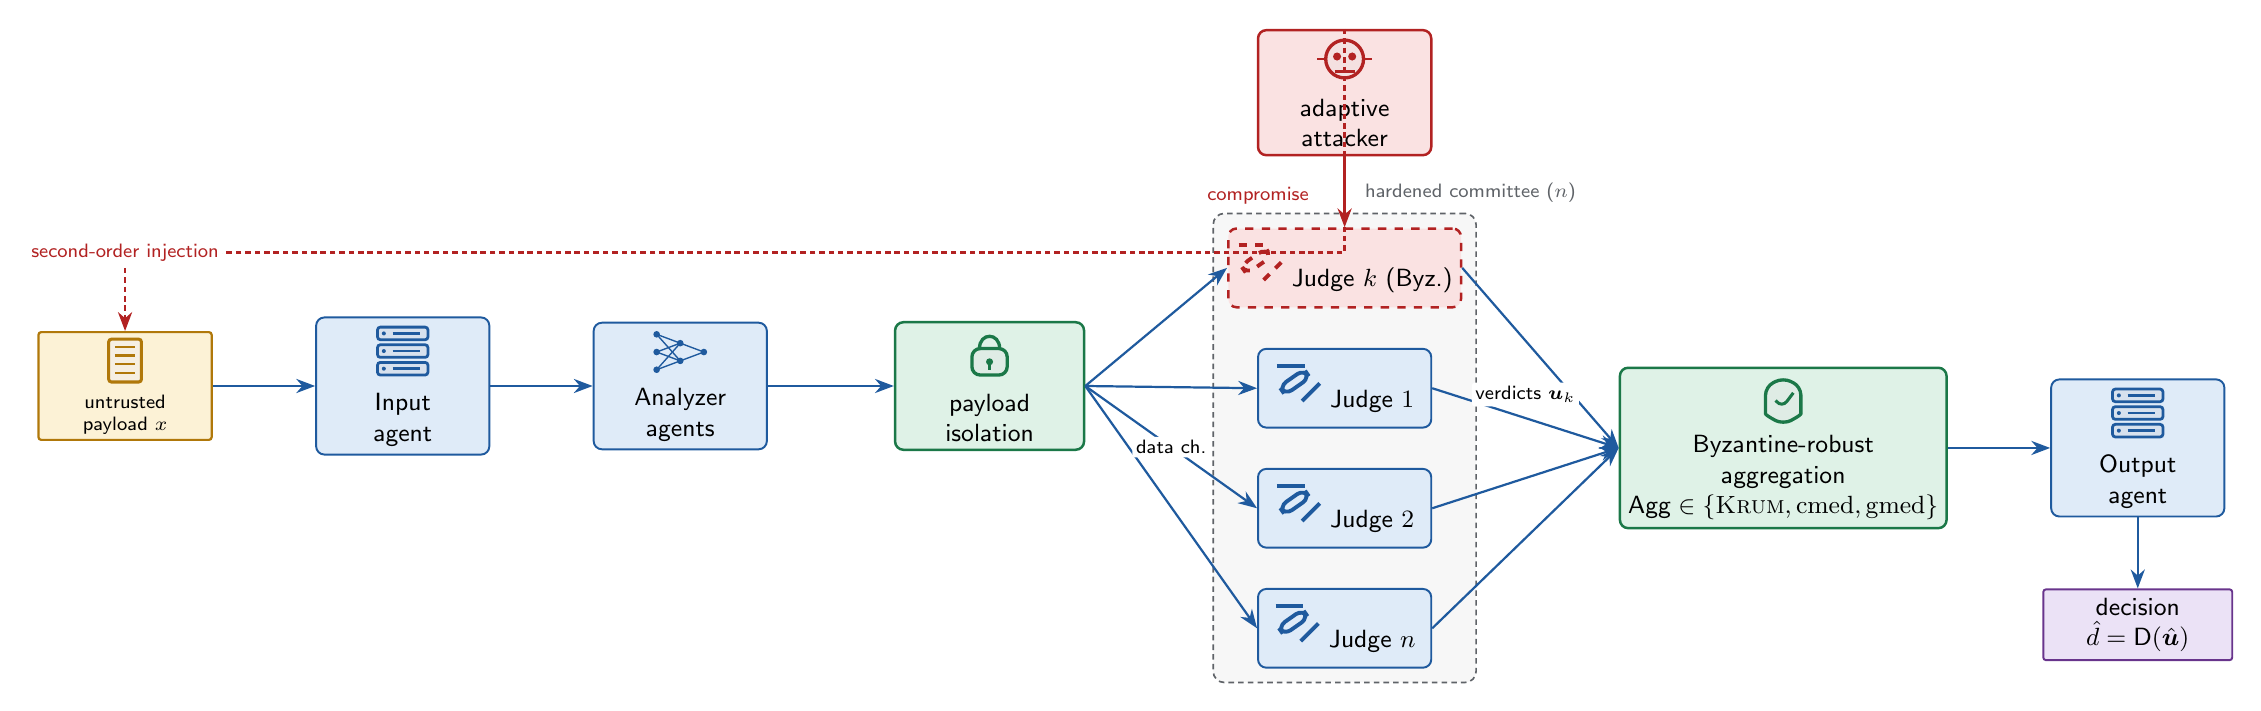
\begin{tikzpicture}[node distance=8mm and 13mm]

% ---- lane 1: honest data path (left to right) ----
\node[payload] (payload) {\icondoc[aegisAmber]\\ untrusted\\ payload $\pay$};
\node[honest, right=of payload] (input) {\iconserver[aegisBlue]\\ Input\\ agent};
\node[honest, right=of input] (analyzer)
  {\iconmodel[aegisBlue]\\ Analyzer\\ agents};

% ---- isolation gate (defense) ----
\node[defense, right=16mm of analyzer] (iso)
  {\iconlock[aegisGreen]\\ payload\\ isolation};

% ---- judge committee (stacked); Byzantine judge placed at top so the
%      compromise arrow drops vertically without crossing other judges ----
\node[byz,    right=18mm of iso, yshift=15mm] (j3) {\iconjudge[aegisRed]\ Judge $k$ (Byz.)};
\node[honest, below=5mm of j3] (j1) {\iconjudge[aegisBlue]\ Judge $1$};
\node[honest, below=5mm of j1] (j2) {\iconjudge[aegisBlue]\ Judge $2$};
\node[honest, below=5mm of j2] (jn) {\iconjudge[aegisBlue]\ Judge $n$};

% committee grouping box
\begin{scope}[on background layer]
  \node[group, fit=(j3)(j1)(j2)(jn),
        label={[grouplabel, xshift=16mm]above:hardened committee ($n$)}] (comm) {};
\end{scope}

% ---- robust aggregator (defense) ----
\node[defense, right=18mm of comm] (agg)
  {\iconshield[aegisGreen]\\ Byzantine-robust\\ aggregation\\ $\Agg\in\{\Krum,\cmed,\gmed\}$};
\node[honest, right=of agg] (out)
  {\iconserver[aegisBlue]\\ Output\\ agent};
\node[theory, below=9mm of out] (dec)
  {decision\\ $\hat d=\dec(\uhat)$};

% ---- attacker (adversarial lane, top), placed above the Byzantine judge ----
\node[adv, above=9mm of j3] (atk) {\iconattacker[aegisRed]\\ adaptive\\ attacker};

% ===== flows =====
% data/model flow (blue)
\draw[dataflow] (payload) -- (input);
\draw[dataflow] (input) -- (analyzer);
\draw[dataflow] (analyzer) -- (iso);
\draw[dataflow] (iso.east) -- (j1.west);
\draw[dataflow] (iso.east) -- (j2.west);
\draw[dataflow] (iso.east) -- (j3.west);
\draw[dataflow] (iso.east) -- (jn.west);
\draw[dataflow] (j1.east) -- (agg.west);
\draw[dataflow] (j2.east) -- (agg.west);
\draw[dataflow] (j3.east) -- (agg.west);
\draw[dataflow] (jn.east) -- (agg.west);
\draw[dataflow] (agg) -- (out);
\draw[dataflow] (out) -- (dec);

% adversarial flow (red): inject payload (routed along the top) + compromise judge k
\draw[advflow] (atk.north) |- ($(payload.north)+(0,10mm)$) -| (payload.north)
  node[elabel,pos=0.25]{second-order injection};
\draw[advflow] (atk.south) -- (j3.north)
  node[elabel,pos=0.55,xshift=-11mm]{compromise};

% control/verdict labels on chips
\node[elabel] at ($(j1.east)!0.5!(agg.west)+(0,3mm)$) {verdicts $\verd_k$};
\node[elabel] at ($(iso.east)!0.5!(j2.west)$) {data ch.};

\end{tikzpicture}}
\caption{The \Aegis\ architecture. Blue: honest data/model flow through Input, Analyzer,
isolation, the hardened judge committee, robust aggregation, and Output. Green:
defensive components (payload isolation and Byzantine-robust verdict aggregation) that
replace AutoDefense's single Coordinator. Red (dashed): the adaptive attacker, which both
injects the untrusted payload (second-order injection against the judges) and compromises
up to $f$ judges (here Judge~$k$). Judges do not communicate with one another; each sends
only its verdict $\verd_k$ to the aggregator. Icons are pure TikZ. Arrow lanes are separated
by colour and dash pattern; labels sit on white chips so no connector crosses text.}
\label{fig:architecture}
\end{figure}


\subsection{The defense agency}
\Aegis is a defensive multi-agent system that adjudicates whether a candidate output may
be released. It comprises (\cref{fig:architecture}):
\begin{itemize}[leftmargin=1.4em,itemsep=2pt,topsep=2pt]
  \item an \textbf{Input agent} that receives the candidate output and any accompanying
        context and places the untrusted content into a structured data channel;
  \item one or more \textbf{Analyzer agents} that extract task-relevant features—the
        apparent user intent and the original instruction/privilege
        hierarchy~\cite{wallace2024instruction}—and attach them to the instruction
        channel as trusted metadata;
  \item a committee of $n$ \textbf{Judge agents} ($1\le n\le 7$ in our study), each a
        hardened LLM~\cite{chen2025secalign,chen2024struq} that reads the isolated
        payload and emits a verdict $v_k$ as in \cref{eq:verdict};
  \item a \textbf{robust aggregator} that replaces AutoDefense's single Coordinator with
        a Byzantine-robust rule $\Agg$ over $\{\verd_k\}$; and
  \item an \textbf{Output agent} that enforces the aggregate decision $\hat d$ (release,
        block, or escalate).
\end{itemize}
The committee is deployed in one of two topologies. In the \emph{parallel} topology the
$n$ judges are queried independently and concurrently; in the \emph{sequential} topology
they are queried in series (relevant only to latency, \cref{sec:complexity}). Judges do
not exchange messages with one another; each communicates only with the aggregator. This
star topology is deliberate: it removes the inter-agent communication channel that
recent attacks exploit~\cite{he2025redteaming,lee2024promptinfection} and confines
adjudication to verdicts the aggregator can robustly combine.

\subsection{Trust boundaries}
Three assets are \emph{trusted}: the aggregation substrate executes $\Agg$ correctly and
non-interactively; the instruction channel delivering the operator's policy is authentic;
and at least $n-f$ judges are honest, with $f$ small enough to satisfy the tolerance
condition of the chosen rule ($2f{+}2<n$ for $\Krum$, $f<n/2$ for median rules). Two
assets are \emph{untrusted}: the payload $\pay$, which may be adversarially crafted, and
up to $f$ judges, which may be compromised or colluding. The aggregator being trusted is
what distinguishes our setting from Byzantine agreement among mutually distrustful
parties~\cite{lamport1982byzantine,castro1999pbft}: we need robust \emph{estimation} of a
verdict, not a consensus protocol. This mirrors the trusted-server assumption of robust
federated aggregation~\cite{blanchard2017krum,yin2018byzantine}, transplanted from
gradients to verdicts.

\subsection{Threat model}
\label{sec:threatmodel}
We adopt the standard security-analysis structure of goal, knowledge, and capability.

\paragraph{Attacker goal.}
Two objectives, dual to each other:
\begin{itemize}[leftmargin=1.4em,itemsep=1pt,topsep=2pt]
  \item \emph{Integrity violation:} cause the agency to \textbf{pass} an output that is
        unsafe or that violates the intended task/instruction
        hierarchy—an evasion, measured by attack success rate under compromise.
  \item \emph{Availability violation:} cause the agency to \textbf{block} benign
        outputs—over-refusal, a denial-of-service against legitimate
        traffic~\cite{zhou2025corba}.
\end{itemize}

\paragraph{Attacker knowledge.}
Black-box to gray-box. The attacker may know the pipeline design, the aggregation rule,
the judges' backbones, and the policy prompt, but not the operator's private randomness
(e.g.\ any per-request nonce used for isolation delimiting). This spans the practical
range from a third party who only submits payloads to an insider who fine-tuned a judge.

\paragraph{Attacker capabilities.}
Three levers, usable in combination:
\begin{enumerate}[leftmargin=1.6em,itemsep=1pt,topsep=2pt]
  \item \textbf{Insider compromise.} Control up to $f$ judges, which then return
        arbitrary, jointly optimised verdict vectors. This is the LLM-committee analogue
        of Byzantine workers~\cite{blanchard2017krum} and of poisoned federated
        clients~\cite{bagdasaryan2020backdoor,fang2020poisoning}.
  \item \textbf{Second-order injection.} Craft the payload $\pay$ so that, in addition to
        being the object under review, it carries instructions aimed at the honest judges
        reading it~\cite{shi2024judgeinjection,greshake2023injection}. Without isolation
        this can flip honest verdicts; with isolation it is reduced to the leakage
        $\varepsilon$ of \cref{def:isolation}.
  \item \textbf{Adaptivity.} Optimise the attack against the specific aggregation rule,
        as adaptive attacks do against robust federated
        aggregators~\cite{fang2020poisoning,baruch2019little,xie2019fall}. Colluding
        judges may coordinate to stay within the honest verdict spread while biasing the
        aggregate.
\end{enumerate}

\paragraph{Collusion.}
Byzantine judges are not independent: they may share a strategy and coordinate their
verdict vectors to move the aggregate as far as the tolerance condition permits. Our
analysis and evaluation treat collusion as the default, not the worst case of an
otherwise-independent fault.

\paragraph{Out of scope.}
We do not defend against (i)~all judges compromised ($f\ge n-f$), which no
minority-tolerance rule can address; (ii)~a correlated failure that affects \emph{every}
judge identically—studied in \cref{sec:theory} as a limiting case that voids the
guarantee, and mitigated but not eliminated by backbone diversity; (iii)~compromise of
the trusted aggregation substrate or the instruction channel; and (iv)~attacks on the
underlying serving infrastructure. \Cref{fig:threat} maps each in-scope lever to the
component it targets and the defense that contains it.

% figures/tikz_threat_privacy_robustness.tex  ->  \cref{fig:threat}
\begin{figure}[t]
\centering
\resizebox{0.98\textwidth}{!}{%
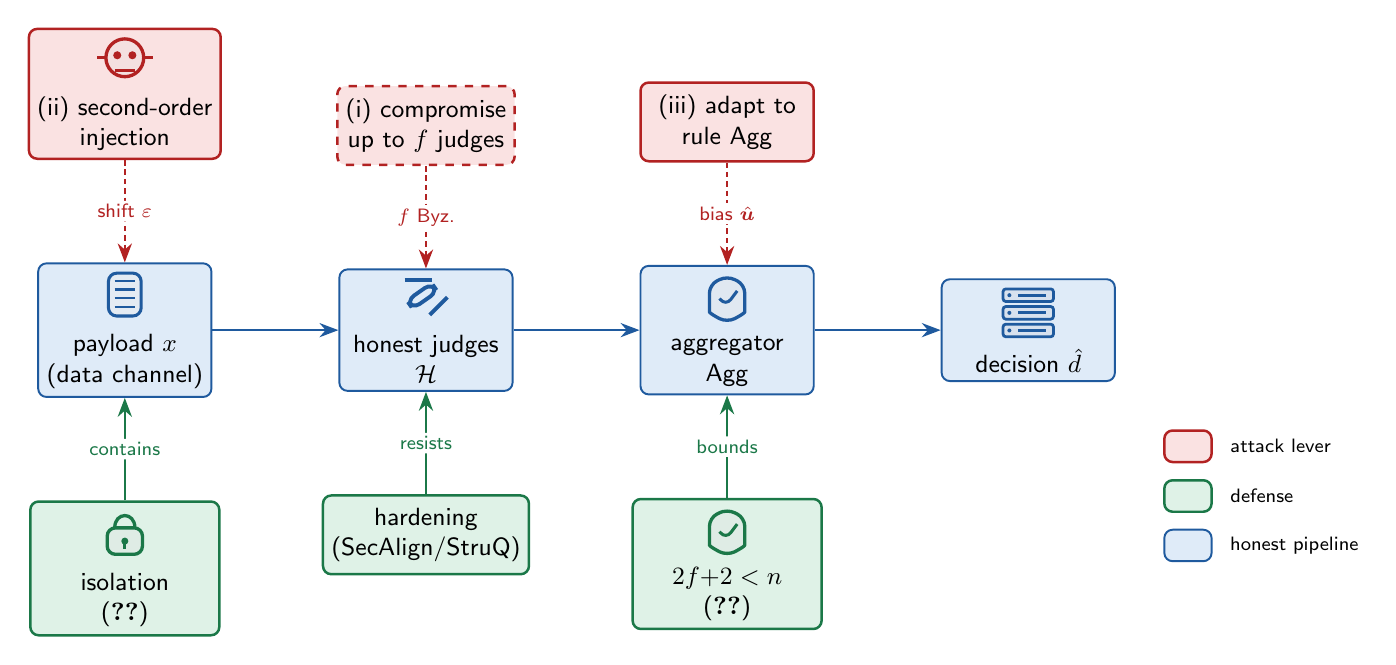
\begin{tikzpicture}[node distance=9mm and 16mm]

% central pipeline spine (honest, blue) -------------------------------
\node[honest] (payload) {\icondoc[aegisBlue]\\ payload $\pay$\\ (data channel)};
\node[honest, right=of payload] (judges) {\iconjudge[aegisBlue]\\ honest judges\\ $\Hset$};
\node[honest, right=of judges] (agg) {\iconshield[aegisBlue]\\ aggregator\\ $\Agg$};
\node[honest, right=of agg] (dec) {\iconserver[aegisBlue]\\ decision $\hat d$};
\foreach \a/\b in {payload/judges, judges/agg, agg/dec}
  \draw[dataflow] (\a) -- (\b);

% attacker levers (red, top) ------------------------------------------
\node[adv, above=13mm of payload] (t2) {\iconattacker[aegisRed]\\ (ii) second-order\\ injection};
\node[byz, above=13mm of judges] (t1) {(i) compromise\\ up to $f$ judges};
\node[adv, above=13mm of agg] (t3) {(iii) adapt to\\ rule $\Agg$};

\draw[advflow] (t2.south) -- (payload.north) node[elabel,midway]{shift $\varepsilon$};
\draw[advflow] (t1.south) -- (judges.north) node[elabel,midway]{$f$ Byz.};
\draw[advflow] (t3.south) -- (agg.north) node[elabel,midway]{bias $\uhat$};

% defenses (green, bottom) --------------------------------------------
\node[defense, below=13mm of payload] (d2) {\iconlock[aegisGreen]\\ isolation\\ (\cref{prop:isolation})};
\node[defense, below=13mm of judges] (d1) {hardening\\ (SecAlign/StruQ)};
\node[defense, below=13mm of agg] (d3) {\iconshield[aegisGreen]\\ $2f{+}2<n$\\ (\cref{thm:integrity})};

\draw[defflow] (d2.north) -- (payload.south) node[elabel,midway]{contains};
\draw[defflow] (d1.north) -- (judges.south) node[elabel,midway]{resists};
\draw[defflow] (d3.north) -- (agg.south) node[elabel,midway]{bounds};

% legend --------------------------------------------------------------
\node[adv, minimum width=6mm, minimum height=4mm, below right=6mm and 6mm of dec] (lgA) {};
\node[right=1mm of lgA, aegissmall] (lgAt) {attack lever};
\node[defense, minimum width=6mm, minimum height=4mm, below=2mm of lgA] (lgD) {};
\node[right=1mm of lgD, aegissmall] {defense};
\node[honest, minimum width=6mm, minimum height=4mm, below=2mm of lgD] (lgH) {};
\node[right=1mm of lgH, aegissmall] {honest pipeline};

\end{tikzpicture}}
\caption{Threat-and-defense map. The honest pipeline spine (blue) runs left to right. Above
it (red), the three composable attacker levers: (i) compromising up to $f$ judges (dashed
Byzantine node), (ii) second-order injection of the payload, and (iii) adapting to the
aggregation rule. Below it (green), the mechanism that contains each lever: isolation for
(ii), judge hardening for the judges, and the $2f{+}2<n$ robust-aggregation guarantee for
(iii). Each attack and defense connects to the single component it acts on; lanes are
separated by colour and dash, and every label sits on a white chip.}
\label{fig:threat}
\end{figure}


\section{Problem Formulation}
\label{sec:problem}

\subsection{The adjudication task}
Let $\pay$ be an inspected payload drawn from a distribution over benign and adversarial
content, and let $y^\star(\pay)\in\{0,1\}$ be the ground-truth label ($1$ if $\pay$ must
be blocked because it is unsafe or violates the intended task/instruction hierarchy,
$0$ otherwise). The agency computes verdicts $\{\verd_k\}_{k\in[n]}$, aggregates them to
$\uhat=\Agg(\verd_1,\dots,\verd_n)$, and outputs $\hat d=\dec(\uhat)$. We evaluate the
agency by two dual error rates, each measured under an adversary that controls up to $f$
judges and the payload:
\begin{align}
  \textsc{asr-uc}(f) &= \Prob\bigl[\hat d = 0 \,\big|\, y^\star(\pay)=1\bigr]
    && \text{(attack success under compromise / evasion)}, \label{eq:asruc}\\
  \textsc{orr}(f)   &= \Prob\bigl[\hat d = 1 \,\big|\, y^\star(\pay)=0\bigr]
    && \text{(over-refusal / availability loss)}. \label{eq:orr}
\end{align}
The probabilities are over the payload distribution, the judges' stochasticity, and the
adversary's choices. \textsc{asr-uc} generalises the jailbreak attack success rate of
AutoDefense~\cite{zeng2024autodefense} to (i)~task-integrity violations and (ii)~the
presence of compromised judges; \textsc{orr} captures the cost the idea flags explicitly,
that a block-biased aggregator harms benign traffic.

\subsection{Design goals}
\begin{description}[leftmargin=0em,itemsep=2pt,topsep=2pt]
  \item[\textnormal{(G1) Decision integrity under a Byzantine minority.}] For $f$ below
        the rule's tolerance, up to $f$ colluding judges must not be able to force
        $\hat d=0$ on a payload the honest committee would block, nor $\hat d=1$ on one it
        would allow. This is the property flagged in the idea as ``to be proven, not
        assumed''; \cref{sec:theory} establishes it under explicit assumptions.
  \item[\textnormal{(G2) Second-order injection containment.}] Instructions embedded in
        the payload must not, on their own, change honest verdicts; the attacker's only
        remaining lever should be to spend from its budget of $f$ compromised judges.
  \item[\textnormal{(G3) Graceful degradation, not brittleness.}] As $f$ grows toward the
        tolerance boundary and as honest verdicts become correlated, \textsc{asr-uc} and
        \textsc{orr} should rise smoothly and predictably, with the dependence
        characterised rather than assumed away.
  \item[\textnormal{(G4) Bounded cost.}] The security gain must be accounted against
        latency and token/API cost, both of which grow with the committee size $n$.
\end{description}

\subsection{What ``secure'' does and does not mean here}
We state a non-claim precisely, because it governs the theory and the evaluation.
A reduction in \textsc{asr-uc}$(f)$ relative to a single model or a plain majority vote is
\emph{evidence of graceful degradation}. It is \emph{not} a proof that the agency is
secure: our guarantees are conditional on assumptions (honest concentration, decision
margin, tolerable correlation) that may fail in deployment, and adaptive attacks are known
to defeat robust aggregators when their assumptions are
violated~\cite{fang2020poisoning,baruch2019little}. We therefore (a)~prove (G1)--(G2)
under assumptions we state in full, (b)~characterise the degradation in (G3) quantitatively,
and (c)~report residual failures and the security-versus-cost frontier (G4) rather than a
single headline number.

\subsection{Threat-to-defense map}
\Cref{tab:threatmap} pins each attacker lever to the design goal and mechanism that
addresses it, and to where it is analysed and tested. The rest of the paper follows this
map.

\begin{table}[t]
\centering
\caption{Threat-to-defense map. Each attacker lever is contained by a specific mechanism,
analysed under specific assumptions, and exercised by a specific attack in the evaluation.}
\label{tab:threatmap}
\small
\begin{tabular}{@{}p{3.0cm}p{2.6cm}p{3.1cm}p{3.4cm}@{}}
\toprule
Attacker lever & Design goal & Mechanism & Analysed / tested by \\
\midrule
Compromise up to $f$ judges & (G1) integrity & Byzantine-robust aggregation
  ($\Krum$/$\cmed$/$\gmed$) & \cref{thm:integrity}; compromised-judge \& colluding attacks \\
Second-order injection of payload & (G2) containment & payload isolation (structured
  data channel) + hardened judges & \cref{def:isolation}, \cref{prop:isolation};
  second-order injection attack \\
Adapt to the aggregation rule & (G1),(G3) & tolerance condition + diversity;
  no reliance on a single aggregator & \cref{thm:integrity}, \cref{prop:correlated};
  adaptive-on-aggregation attack \\
Force over-refusal (availability) & (G1) availability & symmetric robust-aggregation
  guarantee & \cref{cor:availability}; over-refusal measurement \\
Correlated judge failure & (G3) degradation & backbone/prompt diversity; measured
  residual correlation & \cref{prop:correlated}; homogeneous-vs-diverse ablation \\
\bottomrule
\end{tabular}
\end{table}

\section{The \Aegis\ Architecture}
\label{sec:method}

\Aegis instantiates the four components of \cref{sec:intro} as a single pipeline
(\cref{fig:pipeline}). We describe each, then the design rationale that ties them
together.

% figures/tikz_method_pipeline.tex  ->  \cref{fig:pipeline}
\begin{figure}[t]
\centering
\resizebox{\textwidth}{!}{%
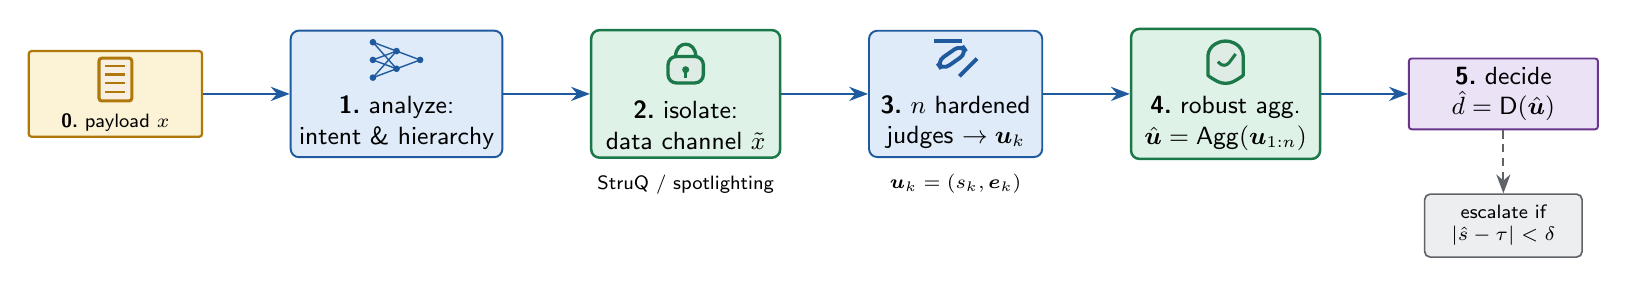
\begin{tikzpicture}[node distance=6mm and 11mm]

\node[payload] (s0) {\icondoc[aegisAmber]\\ \textbf{0.}\ payload $\pay$};
\node[honest, right=of s0] (s1)
  {\iconmodel[aegisBlue]\\ \textbf{1.}\ analyze:\\ intent \& hierarchy};
\node[defense, right=of s1] (s2)
  {\iconlock[aegisGreen]\\ \textbf{2.}\ isolate:\\ data channel $\tilde{\pay}$};
\node[honest, right=of s2] (s3)
  {\iconjudge[aegisBlue]\\ \textbf{3.}\ $n$ hardened\\ judges $\to\verd_k$};
\node[defense, right=of s3] (s4)
  {\iconshield[aegisGreen]\\ \textbf{4.}\ robust agg.\\ $\uhat=\Agg(\verd_{1:n})$};
\node[theory, right=of s4] (s5)
  {\textbf{5.}\ decide\\ $\hat d=\dec(\uhat)$};

% escalate branch
\node[infra, below=8mm of s5] (esc) {escalate if\\ $|\hat s-\thr|<\delta$};

% straight numbered pipeline (blue data flow)
\foreach \a/\b in {s0/s1, s1/s2, s2/s3, s3/s4, s4/s5}
  \draw[dataflow] (\a) -- (\b);
\draw[ctrlflow] (s5.south) -- (esc.north);

% short equation chips under key stages (no crossing)
\node[elabel, below=1.5mm of s3] {$\verd_k=(\score_k,\emb_k)$};
\node[elabel, below=1.5mm of s2] {StruQ / spotlighting};

\end{tikzpicture}}
\caption{The \Aegis\ method pipeline as five numbered, left-to-right stages
(\cref{alg:aegis}). Stage~2 (isolation, green) and stage~4 (robust aggregation, green) are
the defensive additions; stage~3 (blue) is the hardened judge committee. The control-flow
branch (gray, dashed) escalates low-margin cases to review. Short equations are placed on
white chips beneath their stage so no arrow crosses text.}
\label{fig:pipeline}
\end{figure}


\subsection{Payload isolation}
\label{sec:isolation}
The Input agent places the untrusted candidate into a structured data channel that is
lexically and positionally separated from the judges' instruction channel, following the
structured-query design of StruQ~\cite{chen2024struq} and the marking discipline of
spotlighting~\cite{hines2024spotlighting}. Concretely, the payload is wrapped in
reserved, per-request delimiters unknown to the attacker and never interpreted as
control tokens, and the judge is fine-tuned to treat everything in the data channel as
inert evidence to be classified, not as instructions to follow. We formalise the target
property:
\begin{definition}[$\varepsilon$-isolation]
\label{def:isolation}
A judge with verdict distribution $P(\cdot\mid c,\pay)$ given instruction-channel content
$c$ and data-channel payload $\pay$ is \emph{$\varepsilon$-isolated} if for every payload
$\pay$ and every ``injected'' variant $\pay'$ that differs from $\pay$ only by added
instruction-like content,
\begin{equation}
  \sup_{c}\; \operatorname{TV}\!\bigl(P(\cdot\mid c,\pay),\,P(\cdot\mid c,\pay')\bigr)\;\le\;\varepsilon ,
  \label{eq:isolation}
\end{equation}
where $\operatorname{TV}$ is total-variation distance over the verdict $v$. Perfect
isolation is $\varepsilon=0$.
\end{definition}
$\varepsilon$ is an empirical property of a hardened, isolated judge, measured in
\cref{sec:experiments} by the shift in verdicts induced by JudgeDeceiver-style
injections~\cite{shi2024judgeinjection}. Isolation does not make a judge correct; it makes
its verdict insensitive to instructions hidden in what it reads, which is what (G2)
requires.

\subsection{Hardened judges}
\label{sec:hardened}
Each judge is an LLM fine-tuned for injection resistance by preference
optimisation~\cite{chen2025secalign,rafailov2023dpo} and structured-input
training~\cite{chen2024struq}, on top of an aligned backbone~\cite{ouyang2022instructgpt,bai2022constitutional,touvron2023llama2}.
A judge outputs the verdict of \cref{eq:verdict}: a decision, a score calibrated by
temperature scaling~\cite{guo2017calibration} so that scores are comparable across judges,
and a rationale embedding from a fixed sentence
encoder~\cite{reimers2019sentencebert,gao2021simcse} that places the free-text
justification in a shared semantic space. The embedding is what lets robust aggregation
see \emph{how} a judge reasoned, not only \emph{what} it decided, so that a colluding
judge that reports the honest decision but a manipulated rationale is still an outlier in
$\R^d$.

\subsection{Byzantine-robust verdict aggregation}
\label{sec:aggregation}
The aggregator replaces the single Coordinator with a robust rule $\Agg$ over
$\{\verd_k\}$. We support the three rules of \cref{sec:prelim}. $\cmed$ and $\gmed$
tolerate $f<n/2$ and are cheap; $\Krum$ tolerates $f$ with $2f{+}2<n$ and returns an
\emph{actual} judge verdict (useful when the operator wants an attributable rationale).
The aggregate verdict $\uhat$ yields the decision $\hat d=\dec(\uhat)$. The design choice
that makes this meaningful is aggregating in the \emph{semantic verdict space} $\R^d$
rather than over decisions alone: a plain majority vote sees only $d_k$ and is blind to a
colluder that votes with the honest majority while skewing scores to shift a downstream
threshold or to poison an audit log; aggregating $(\score_k,\emb_k)$ exposes such a
colluder as a geometric outlier.

\subsection{Task-integrity generalisation}
\label{sec:taskintegrity}
The verdict target is lifted from ``is this content harmful?'' to ``does this output
violate the intended task or privilege hierarchy?''~\cite{wallace2024instruction}. The
Analyzer agents supply the honest task specification on the instruction channel; each
judge decides whether the payload, treated as inert data, is consistent with that
specification. This is what turns a jailbreak filter into a prompt-injection filter: an
output can be perfectly harmless in isolation yet still constitute a successful injection
if it obeys an instruction that was smuggled through the data channel rather than issued
by the operator~\cite{greshake2023injection,liu2024formalizing}.

\subsection{Design rationale: why all four are needed}
\label{sec:rationale}
The components are not independent add-ons; each closes a gap the others leave open, and
this is the core of our novelty argument.
\begin{itemize}[leftmargin=1.4em,itemsep=2pt,topsep=2pt]
  \item \emph{Hardened judges alone} are the single-model baseline
        (SecAlign~\cite{chen2025secalign}). They have no co-defender to collude and no
        aggregator to subvert—so they cannot express, let alone defend, the insider
        threat.
  \item \emph{Robust aggregation alone}, over un-isolated judges, is defeated by
        second-order injection: an attacker who can flip honest verdicts through the data
        channel moves the honest majority itself, and no minority-tolerance rule helps
        once the honest inputs are corrupted~\cite{shi2024judgeinjection}.
  \item \emph{Isolation alone}, over a single un-aggregated judge, still falls to a single
        compromised judge, because there is no committee.
  \item \emph{Aggregation over decisions alone} (plain majority vote) is blind to
        score/rationale manipulation and, as \cref{prop:correlated} shows, collapses under
        correlated failure.
\end{itemize}
The combination gives (G1) from aggregation, (G2) from isolation plus hardening, and (G3)
from the diversity requirement that aggregation's assumptions impose. \Cref{fig:pipeline}
shows the flow; \cref{sec:algorithm} gives the procedure; \cref{sec:theory} proves what
the combination buys and states precisely where it stops.

\section{Algorithm}
\label{sec:algorithm}

\Cref{alg:aegis} states the \Aegis\ adjudication procedure, and \cref{alg:agg} the robust
aggregation subroutines. The pipeline is a single non-interactive pass: analyze, isolate,
query $n$ hardened judges (in parallel), aggregate their verdict vectors robustly, and
enforce the decision. No judge sees another judge's verdict, so a compromised judge cannot
influence honest ones; its only reach is the aggregator, which is robust by construction.

\begin{algorithm}[t]
\caption{\Aegis\ adjudication}
\label{alg:aegis}
\begin{algorithmic}[1]
\Require payload $\pay$; policy prompt $c_0$; committee of $n$ hardened judges
  $\{J_k\}$; aggregation rule $\Agg\in\{\Krum,\cmed,\gmed\}$; threshold $\thr$;
  encoders (score calibrator $g$, sentence encoder $\phi$)
\Ensure decision $\hat d\in\{\text{allow},\text{block},\text{escalate}\}$
\State $(\text{intent},\text{hierarchy}) \gets \textsc{Analyze}(\pay)$
  \Comment{trusted task spec on instruction channel}
\State $c \gets c_0 \,\Vert\, \text{intent}\,\Vert\,\text{hierarchy}$
\State $\tilde{\pay} \gets \textsc{Isolate}(\pay)$
  \Comment{wrap payload in per-request delimiters; data channel only}
\For{$k = 1$ \textbf{to} $n$ \textbf{in parallel}}
  \State $(d_k, \text{raw}_k, \text{rationale}_k) \gets J_k(\text{instruction}{=}c,\ \text{data}{=}\tilde{\pay})$
  \State $\score_k \gets g(\text{raw}_k)$; \quad $\emb_k \gets \phi(\text{rationale}_k)$
    \Comment{calibrated score; rationale embedding}
  \State $\verd_k \gets (\score_k, \emb_k)\in\R^{d}$
\EndFor
\State $\uhat \gets \Agg(\verd_1,\dots,\verd_n)$
  \Comment{robust aggregation in verdict space (\cref{alg:agg})}
\State $\hat s \gets \pi_1(\uhat)$
\If{$|\hat s - \thr| < \delta$} \Return \textbf{escalate}
  \Comment{low-margin case: defer to human/secondary review}
\ElsIf{$\hat s \ge \thr$} \Return \textbf{block}
\Else{} \ \Return \textbf{allow}
\EndIf
\end{algorithmic}
\end{algorithm}

\begin{algorithm}[t]
\caption{Robust aggregation subroutines $\Agg(\verd_1,\dots,\verd_n)$}
\label{alg:agg}
\begin{algorithmic}[1]
\Function{CoordinateMedian}{$\verd_1,\dots,\verd_n$}
  \For{$j = 1$ \textbf{to} $d$}
    \State $\pi_j(\uhat) \gets \operatorname{median}\{\pi_j(\verd_1),\dots,\pi_j(\verd_n)\}$
  \EndFor
  \State \Return $\uhat$
\EndFunction
\Statex
\Function{GeometricMedian}{$\verd_1,\dots,\verd_n$; tolerance $\eta$}
  \State $\bm y \gets \tfrac1n\sum_k \verd_k$
  \Comment{Weiszfeld iteration~\cite{pillutla2022rfa}}
  \Repeat
    \State $w_k \gets 1/\max(\lVert \bm y - \verd_k\rVert,\ \eta)$ for each $k$
    \State $\bm y \gets \bigl(\sum_k w_k \verd_k\bigr)/\bigl(\sum_k w_k\bigr)$
  \Until{convergence}
  \State \Return $\bm y$
\EndFunction
\Statex
\Function{Krum}{$\verd_1,\dots,\verd_n$; assumed faults $f$}
  \For{$k = 1$ \textbf{to} $n$}
    \State $\mathcal N_k \gets$ indices of the $n-f-2$ nearest $\verd_j$ ($j\neq k$) to $\verd_k$
    \State $\text{score}(k) \gets \sum_{j\in\mathcal N_k}\lVert \verd_k - \verd_j\rVert^2$
  \EndFor
  \State \Return $\verd_{k^\star}$ where $k^\star = \arg\min_k \text{score}(k)$
\EndFunction
\end{algorithmic}
\end{algorithm}

\paragraph{Remarks on the algorithm.}
The \emph{escalate} branch (\cref{alg:aegis}, line~11) implements graceful degradation at
the decision level: when the robust aggregate lands within $\delta$ of the threshold—the
regime where \cref{thm:integrity} cannot certify the decision—the agency defers rather
than guesses, converting an uncertain automated verdict into a review request. Setting
$\delta=0$ recovers a pure allow/block agency. The three subroutines expose the
security--cost trade-off of \cref{sec:complexity}: $\cmed$ is $O(nd)$ per request (with an
$O(n\log n)$ selection per coordinate), $\gmed$ is $O(Tnd)$ for $T$ Weiszfeld iterations,
and $\Krum$ is $O(n^2 d)$ from its pairwise distances. All three are negligible beside the
$n$ LLM calls, which dominate cost and are the reason $n$ is kept small.

\section{Theoretical Analysis}
\label{sec:theory}

We establish the decision-integrity property (G1) for robust verdict aggregation under
explicit assumptions, its availability dual, the second-order-injection containment (G2),
and the correlated-failure degradation (G3). Proofs of the two results marked with a
dagger ($\dagger$) are complete and given in \cref{app:proofs}; the remaining statements
are labelled as proof sketches or as restatements of cited results, and none is presented
as more than it is. \Cref{fig:theory} shows the dependency structure.

% figures/tikz_theory_diagram.tex  ->  \cref{fig:theory}
\begin{figure}[t]
\centering
\resizebox{0.98\textwidth}{!}{%
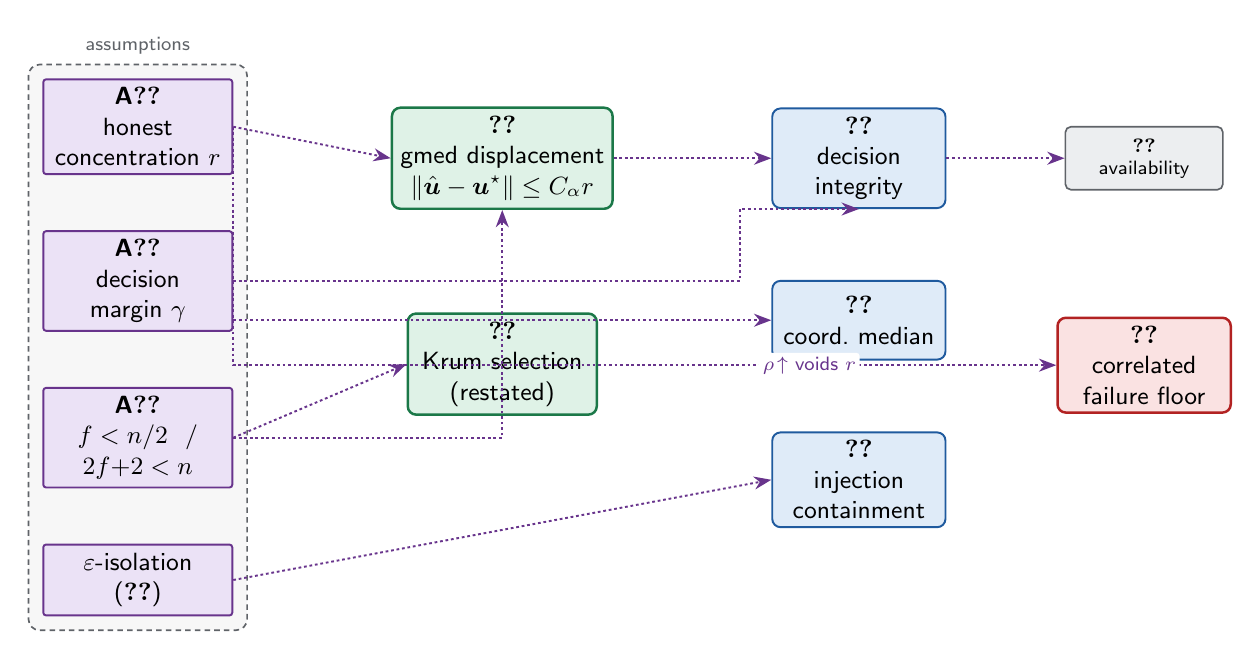
\begin{tikzpicture}[node distance=7mm and 15mm]

% ---- assumptions (purple, left column) ----
\node[theory] (a1) {\textbf{A\ref{ass:concentration}}\\ honest\\ concentration $r$};
\node[theory, below=of a1] (a2) {\textbf{A\ref{ass:margin}}\\ decision\\ margin $\gamma$};
\node[theory, below=of a2] (a3) {\textbf{A\ref{ass:fraction}}\\ $f<n/2$ \ /\\ $2f{+}2<n$};
\node[theory, below=of a3] (aiso) {$\varepsilon$-isolation\\ (\cref{def:isolation})};

\begin{scope}[on background layer]
  \node[group, fit=(a1)(a2)(a3)(aiso), label={[grouplabel]above:assumptions}] {};
\end{scope}

% ---- lemmas (middle) ----
\node[defense, right=20mm of a1, yshift=-4mm] (lem1)
  {\textbf{\cref{lem:gmedrobust}}\\ gmed displacement\\ $\lVert\uhat-\ustar\rVert\le C_\alpha r$};
\node[defense, below=13mm of lem1] (lem2)
  {\textbf{\cref{lem:krum}}\\ Krum selection\\ (restated)};

% ---- theorems (right) ----
\node[honest, right=20mm of lem1] (thm1)
  {\textbf{\cref{thm:integrity}}\\ decision\\ integrity};
\node[honest, below=9mm of thm1] (propc)
  {\textbf{\cref{prop:cmed}}\\ coord.\ median};
\node[honest, below=9mm of propc] (propiso)
  {\textbf{\cref{prop:isolation}}\\ injection\\ containment};

% ---- corollary / outcomes (far right) ----
\node[infra, right=15mm of thm1] (cor)
  {\textbf{\cref{cor:availability}}\\ availability};
\node[adv, below=16mm of cor] (corr)
  {\textbf{\cref{prop:correlated}}\\ correlated\\ failure floor};

% ===== theory dependency flow (purple dashed) =====
\draw[theoryflow] (a1.east) -- (lem1.west);
\draw[theoryflow] (a3.east) -| (lem1.south);
\draw[theoryflow] (a3.east) -- (lem2.west);
\draw[theoryflow] (lem1.east) -- (thm1.west);
\draw[theoryflow] (a2.east) -| ($(thm1.south west)+(-4mm,0)$) |- (thm1.south);
\draw[theoryflow] (a1.east) |- (propc.west);
\draw[theoryflow] (aiso.east) -- (propiso.west);
\draw[theoryflow] (thm1.east) -- (cor.west);
\draw[theoryflow] (a1.east) |- (corr.west)
  node[elabel,pos=0.85]{$\rho\!\uparrow$ voids $r$};

\end{tikzpicture}}
\caption{Theory dependency graph. Assumptions (purple) feed lemmas (green), which feed
theorems and propositions (blue); the availability corollary (gray) and the correlated-failure
floor (red, a limiting-case impossibility that \emph{voids} the concentration assumption)
are downstream. Routed orthogonal connectors avoid diagonal clutter; the only annotated
edge notes that rising error correlation $\rho$ invalidates the honest radius $r$ that
\cref{lem:gmedrobust,thm:integrity} require.}
\label{fig:theory}
\end{figure}


\subsection{Assumptions}
\begin{assumption}[Honest concentration]
\label{ass:concentration}
There is a reference verdict $\ustar\in\R^d$ and a radius $r\ge 0$ such that every honest
judge's verdict vector satisfies $\lVert \verd_k-\ustar\rVert\le r$ for all $k\in\Hset$.
\end{assumption}

\begin{assumption}[Decision margin]
\label{ass:margin}
The reference score is bounded away from the threshold: $|\pi_1(\ustar)-\thr|\ge\gamma$
for some margin $\gamma>0$, and the reference decision equals the ground truth,
$\dec(\ustar)=y^\star(\pay)$.
\end{assumption}

\begin{assumption}[Tolerable Byzantine fraction]
\label{ass:fraction}
For median-type rules ($\cmed,\gmed$), $f<n/2$; for $\Krum$, $2f{+}2<n$.
\end{assumption}

\begin{remark}
\Cref{ass:concentration,ass:margin} are the substantive assumptions and they are
\emph{empirical claims about honest judges}, not mathematical conveniences. Honest
concentration can fail if honest judges genuinely disagree (a hard, ambiguous payload) or
if they share a systematic bias~\cite{zheng2023judging,wang2023notfair}; the margin can be
small near policy boundaries. We measure $r$ and $\gamma$ in \cref{sec:experiments} rather
than assume favourable values, and \cref{prop:correlated} treats the case where
concentration degrades because honest errors are correlated.
\end{remark}

\subsection{Robustness of the aggregate verdict}
The engine of (G1) is a deterministic robustness bound for the geometric median. We state
it and give the complete proof in \cref{app:proofs}.

\begin{lemma}[Geometric-median displacement$^{\dagger}$]
\label{lem:gmedrobust}
Let $\verd_1,\dots,\verd_n\in\R^d$, and suppose a subset $\Hset$ with $|\Hset|=n-f$
satisfies $\lVert\verd_k-\ustar\rVert\le r$ for all $k\in\Hset$. If $f<n/2$, then the
geometric median $\uhat=\gmed(\verd_1,\dots,\verd_n)$ satisfies
\begin{equation}
  \lVert \uhat-\ustar\rVert \;\le\; C_\alpha\, r,
  \qquad C_\alpha \;=\; \frac{2(n-f)}{\,n-2f\,}\;=\;\frac{2(1-\alpha)}{1-2\alpha},
  \label{eq:gmedbound}
\end{equation}
where $\alpha=f/n<\tfrac12$. The bound holds for arbitrary (adversarially chosen)
Byzantine verdicts $\{\verd_k\}_{k\in\Bset}$.
\end{lemma}

\begin{remark}
$C_\alpha$ is finite and increasing on $[0,\tfrac12)$, diverging as $\alpha\to\tfrac12$:
$C_0=2$, $C_{1/4}=3$, $C_{1/3}=4$. Thus tolerance is graceful, not binary—the aggregate
can be pushed further as the Byzantine fraction approaches one half, exactly the graceful
degradation (G3) asks for. The constant matches the breakdown behaviour of multivariate
location estimators~\cite{lopuhaa1991breakdown,minsker2015geometric}. We are careful
\emph{not} to claim this constant is optimal or that it is a matching bound; it is a
sufficient displacement bound.
\end{remark}

\subsection{Decision integrity and availability}
\begin{theorem}[Decision integrity under a Byzantine minority$^{\dagger}$]
\label{thm:integrity}
Under \cref{ass:concentration,ass:margin} and \cref{ass:fraction} with a median-type rule,
if the margin dominates the displacement,
\begin{equation}
  \gamma \;>\; C_\alpha\, r ,
  \label{eq:integritycond}
\end{equation}
then the aggregate decision equals the honest reference decision,
$\dec(\uhat)=\dec(\ustar)=y^\star(\pay)$, for every choice of the $f$ Byzantine verdicts.
Consequently up to $f$ colluding judges can neither force a block payload to pass nor a
benign payload to be blocked.
\end{theorem}

\begin{corollary}[Availability]
\label{cor:availability}
Under the hypotheses of \cref{thm:integrity} the over-refusal event $\{\hat d=1\mid
y^\star=0\}$ cannot be induced by the $f$ Byzantine judges: the guarantee is symmetric in
the two decision directions. Hence robust aggregation addresses the availability goal of
\cref{sec:problem} on the same terms as the integrity goal.
\end{corollary}

\Cref{thm:integrity} is the precise form of the property the idea flagged as
``to be proven, not assumed.'' Its content is conditional: robust aggregation converts a
minority of arbitrary Byzantine verdicts into a bounded displacement of the aggregate, and
a sufficient decision margin converts a bounded displacement into an unchanged decision.
The condition $\gamma>C_\alpha r$ is where the empirical burden sits—it is satisfied only
if honest judges concentrate tightly ($r$ small) relative to their distance from the
policy boundary ($\gamma$ large), which is precisely what backbone diversity and hardening
are meant to deliver and what \cref{sec:experiments} measures.

\subsection{Coordinate-wise median and Krum}
\begin{proposition}[Coordinate-median integrity]
\label{prop:cmed}
Under \cref{ass:concentration,ass:fraction} with $f<n/2$, each coordinate of
$\uhat=\cmed(\verd_1,\dots,\verd_n)$ lies within the range of the honest coordinates:
$\min_{k\in\Hset}\pi_j(\verd_k)\le \pi_j(\uhat)\le \max_{k\in\Hset}\pi_j(\verd_k)$ for all
$j$. In particular $|\pi_1(\uhat)-\pi_1(\ustar)|\le r$, and \cref{eq:integritycond} with
$C_\alpha$ replaced by $1$ suffices for \cref{thm:integrity} to hold for the score
coordinate.
\end{proposition}
\begin{proof}[Proof sketch]
With $f<n/2$ Byzantine values among $n$, the median order statistic of each coordinate is
bracketed by two honest order statistics, hence lies in the honest range; the
score-coordinate bound and the margin argument then follow as in \cref{thm:integrity}. The
full argument is a one-dimensional specialisation and is given in \cref{app:proofs}. This
recovers the tolerance behaviour of coordinate-wise median in Byzantine
learning~\cite{yin2018byzantine}.
\end{proof}

\begin{lemma}[Krum selection, restated from~\cite{blanchard2017krum}]
\label{lem:krum}
Under \cref{ass:fraction} with $2f{+}2<n$, the vector selected by $\Krum$ has, in
expectation over honest stochasticity, squared distance to the honest barycenter bounded
by a constant multiple of the honest variance; in particular a Byzantine minority cannot
force $\Krum$ to select a vector arbitrarily far from the honest verdicts.
\end{lemma}
\begin{remark}
\Cref{lem:krum} is a restatement of the guarantee of Blanchard et
al.~\cite{blanchard2017krum} adapted to our verdict space; we do not reprove it. Two
caveats are transplanted with it. First, the guarantee bounds distance to the honest
barycenter, so it feeds \cref{thm:integrity} only under \cref{ass:concentration} with a
possibly larger effective $r$. Second, single-selection rules such as $\Krum$ can behave
poorly in high dimension~\cite{mhamdi2018bulyan}; because our verdict space is
low-dimensional after embedding compression ($d=1+m$ with modest $m$), and because
$\cmed$/$\gmed$ avoid the single-selection pathology, we treat $\Krum$ as one option among
three rather than the default.
\end{remark}

\subsection{Second-order injection containment}
\begin{proposition}[Isolation containment]
\label{prop:isolation}
Suppose every honest judge is $\varepsilon$-isolated (\cref{def:isolation}) and let a
second-order injection alter the payload from $\pay$ to $\pay'$. Then the injection changes
the decision of any fixed honest judge with probability at most $\varepsilon$, and by a
union bound it changes more than $t$ honest decisions with probability at most
$\binom{n-f}{t+1}\varepsilon^{\,t+1}$ under independent judge draws. In the limit
$\varepsilon\to 0$ (perfect isolation), a second-order injection that does not compromise a
judge's parameters leaves all honest verdicts unchanged, so the attacker's only remaining
lever is to spend from its budget of $f$ compromised judges, which is governed by
\cref{thm:integrity}.
\end{proposition}
\begin{proof}[Proof sketch]
The per-judge bound is immediate from \cref{def:isolation}: total-variation distance
$\varepsilon$ bounds the change in probability of any event, including the decision event.
The union/count bound assumes honest judges respond independently to the injection, which
holds when their randomness is independent; correlated responses are exactly the regime of
\cref{prop:correlated}. The $\varepsilon\to0$ statement is the definition of perfect
isolation. See \cref{app:proofs}.
\end{proof}
\begin{remark}
\Cref{prop:isolation} is conditional on the measured leakage $\varepsilon$; it does not
assert $\varepsilon=0$ in practice. Its role is to separate two attack channels that
un-isolated pipelines conflate: without isolation, a payload injection can move honest
verdicts \emph{for free} (outside the Byzantine budget), defeating any minority-tolerance
rule; with isolation, injection is priced into the budget $f$ that
\cref{thm:integrity} already handles. This is the formal content of the claim that
isolation ``closes the surface the defense creates by reading untrusted text.''
\end{remark}

\subsection{Correlated failure: when the guarantee is vacuous}
\Cref{ass:concentration} presumes honest judges cluster near $\ustar$. If they instead
fail \emph{together}, the honest inputs to the aggregator are themselves wrong and no
robust rule can recover the correct decision. We make the dependence on correlation
quantitative for the decision-level (majority) view, which upper-bounds what any rule
using only decisions can achieve.

\begin{proposition}[Correlated honest failure]
\label{prop:correlated}
Model the honest judges' correctness indicators $\{Z_k\}_{k\in\Hset}$, $Z_k=\mathbf 1\{J_k
\text{ decides correctly}\}$, as exchangeable Bernoulli variables with mean
$\mu=\Prob[Z_k=1]$ and pairwise correlation $\rho\in[0,1]$. Let $\bar Z=\frac1{n-f}
\sum_{k\in\Hset}Z_k$ be the honest correct fraction. Then
\begin{equation}
  \E[\bar Z]=\mu,\qquad
  \operatorname{Var}(\bar Z)=\mu(1-\mu)\!\left[\frac{1-\rho}{\,n-f\,}+\rho\right],
  \label{eq:corrvar}
\end{equation}
so as $n\to\infty$, $\operatorname{Var}(\bar Z)\to \mu(1-\mu)\,\rho>0$ for any $\rho>0$.
Consequently, if $\mu<\tfrac12$ (honest judges are more often wrong than right on a class
of payloads), adding judges does not drive the probability of a correct honest majority to
one; and for $\rho>0$ the honest majority fails with probability bounded below by a
constant independent of $n$ (Chebyshev, \cref{app:proofs}). Backbone/prompt diversity is
the mechanism that reduces $\rho$; the ceiling in \cref{eq:corrvar} is why diversity is a
\emph{requirement}, not an optimisation.
\end{proposition}
\begin{remark}
\Cref{prop:correlated} formalises the idea's warning that ``Krum tolerance is vacuous if
all judges fail identically'' ($\rho\to1$ collapses the committee to a single effective
judge) and that diversity is needed to make the committee more than a single point of
failure. It also explains why plain majority vote and any verdict-space rule share the same
failure mode at the decision level: robustness to a Byzantine \emph{minority} cannot
substitute for correctness of the honest \emph{majority}. This is a limiting-case analysis,
not a defense; it is exactly the residual failure the idea insists on reporting.
\end{remark}

\subsection{Summary of guarantees}
\Cref{tab:guarantees} collects the results, their assumptions, and their status. The two
complete proofs (\cref{lem:gmedrobust,thm:integrity}) are what establish (G1); the
remaining statements support (G2), the median/Krum variants, and the honest boundary of
the whole approach.

\begin{table}[t]
\centering
\caption{Guarantees, assumptions, and proof status. ``Complete'' proofs appear in
\cref{app:proofs}; ``restated'' results are cited, not reproven; ``sketch'' proofs give the
argument with the routine specialisation deferred to the appendix.}
\label{tab:guarantees}
\small
\begin{tabular}{@{}p{3.2cm}p{4.4cm}p{2.2cm}p{2.4cm}@{}}
\toprule
Result & Assumptions & Goal & Status \\
\midrule
\cref{lem:gmedrobust} (gmed displacement) & concentration; $f<n/2$ & (G1) & complete \\
\cref{thm:integrity} (integrity) & concentration; margin $\gamma>C_\alpha r$; $f<n/2$ & (G1) & complete \\
\cref{cor:availability} (availability) & as \cref{thm:integrity} & (G1) avail. & complete (corollary) \\
\cref{prop:cmed} (coordinate median) & concentration; $f<n/2$ & (G1) & sketch \\
\cref{lem:krum} (Krum) & $2f{+}2<n$ & (G1) & restated~\cite{blanchard2017krum} \\
\cref{prop:isolation} (isolation) & $\varepsilon$-isolation & (G2) & sketch \\
\cref{prop:correlated} (correlated failure) & exchangeable honest errors, correlation $\rho$ & (G3) & complete (limiting case) \\
\bottomrule
\end{tabular}
\end{table}

\section{Complexity and the Security--Cost Frontier}
\label{sec:complexity}

\Aegis buys robustness by running a committee, and the idea is explicit that the cost of
that committee may be unattractive at small $n$. We make the cost quantitative and pair it
with the tolerance it purchases, so the trade-off is stated rather than hidden.

\subsection{Token and API cost}
Each request issues one hardened-judge call per committee member plus the Analyzer calls.
Let $\ell_{\text{in}}$ and $\ell_{\text{out}}$ be the per-judge input and output token
counts. The token cost per adjudication is
\begin{equation}
  \text{Tokens}(n) \;=\; n\,(\ell_{\text{in}}+\ell_{\text{out}}) \;+\; \text{Tokens}_{\text{analyze}},
  \label{eq:tokencost}
\end{equation}
i.e.\ \emph{linear} in the committee size $n$, since judges are independent and the payload
is broadcast unchanged. Payload isolation adds only the fixed delimiter overhead. This
linearity is the cost the idea asks to quantify, and it is the reason $n$ is restricted to
the range $1$--$7$: the token bill grows in lockstep with $n$ while, by \cref{lem:gmedrobust},
the tolerated fault count grows only as $\lfloor (n-1)/2\rfloor$ (median rules) or
$\lfloor (n-2)/2\rfloor$ (Krum).

\subsection{Latency}
In the parallel topology the judge calls overlap, so wall-clock latency is
\begin{equation}
  \text{Lat}_{\parallel}(n) \;=\; \max_{k\in[n]} \text{lat}(J_k) \;+\; \text{lat}(\Agg) \;+\; \text{lat}_{\text{analyze}},
  \label{eq:latpar}
\end{equation}
dominated by the slowest judge plus a small aggregation term; in the sequential topology it
is $\sum_k \text{lat}(J_k)+\text{lat}(\Agg)$, linear in $n$. The idea notes latency is
``linear in the number of agents''; \cref{eq:latpar} shows this is the \emph{sequential}
worst case and that parallel deployment reduces the judge contribution to a constant in $n$
(at unchanged token cost), trading hardware concurrency for latency.

\subsection{Aggregation cost}
The three rules cost, per request, $O(nd)$ with an $O(n\log n)$ per-coordinate selection for
$\cmed$; $O(Tnd)$ for $\gmed$ with $T$ Weiszfeld iterations~\cite{pillutla2022rfa}; and
$O(n^2 d)$ for $\Krum$ from its pairwise distances~\cite{blanchard2017krum}. With $n\le 7$
and modest embedding dimension $d=1+m$, all three are dominated by the LLM calls of
\cref{eq:tokencost} and contribute negligibly to latency.

\subsection{The frontier}
Define the \emph{Byzantine tolerance fraction} $\alpha^\star(n)=\lfloor(n-1)/2\rfloor/n$ for
median rules. \Cref{tab:cost} tabulates tolerance against the multiplicative token cost
$n$. The security gain is discrete and, at small $n$, coarse: moving from $n=3$ (tolerates
$f=1$) to $n=5$ (tolerates $f=2$) doubles neither cost-effectiveness nor tolerance cleanly.
Whether a given operating point is worthwhile is an empirical question about the deployment's
threat level and latency budget, which \cref{sec:experiments} is designed to answer rather
than to presuppose.

\begin{table}[t]
\centering
\caption{Security--cost frontier for median-type aggregation. Tolerance is the maximum $f$
with $f<n/2$; token cost is the multiple of a single-judge call from \cref{eq:tokencost}
(Analyzer overhead excluded). Small committees tolerate very few faults, the feasibility
risk the idea flags as an open empirical question.}
\label{tab:cost}
\small
\begin{tabular}{@{}cccc@{}}
\toprule
Committee $n$ & Max tolerated $f$ & Tolerance fraction $\alpha^\star$ & Token cost (\(\times\) single judge) \\
\midrule
1 & 0 & $0.00$ & $1$ \\
2 & 0 & $0.00$ & $2$ \\
3 & 1 & $0.33$ & $3$ \\
4 & 1 & $0.25$ & $4$ \\
5 & 2 & $0.40$ & $5$ \\
6 & 2 & $0.33$ & $6$ \\
7 & 3 & $0.43$ & $7$ \\
\bottomrule
\end{tabular}
\end{table}

\section{Experimental Design}
\label{sec:experiments}

This section specifies the evaluation protocol. \textbf{The numerical entries in
\cref{tab:main,tab:ablation} and the curves in \cref{fig:results} are placeholders that
encode expected trends and fix the measurement procedure; they are not experimental
results and must be replaced with measured values before submission.} No superiority claim
is made on their basis. \Cref{fig:expsetup} summarises the design.

% figures/tikz_experimental_setup.tex  ->  \cref{fig:expsetup}
\begin{figure}[t]
\centering
\resizebox{\textwidth}{!}{%
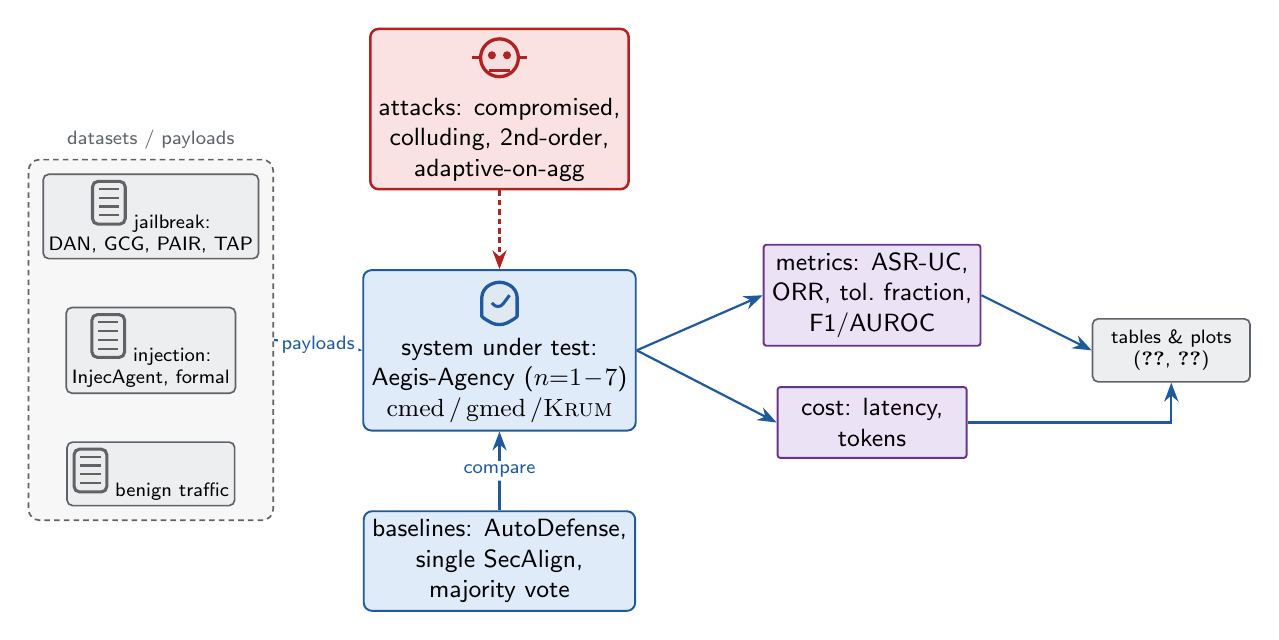
\begin{tikzpicture}[node distance=6mm and 14mm]

% ---- inputs: datasets ----
\node[infra] (d1) {\icondoc[aegisGray]\ jailbreak:\\ DAN, GCG, PAIR, TAP};
\node[infra, below=of d1] (d2) {\icondoc[aegisGray]\ injection:\\ InjecAgent, formal};
\node[infra, below=of d2] (d3) {\icondoc[aegisGray]\ benign traffic};
\begin{scope}[on background layer]
  \node[group, fit=(d1)(d2)(d3), label={[grouplabel]above:datasets / payloads}] (din) {};
\end{scope}

% ---- system under test ----
\node[honest, right=16mm of d2] (sut)
  {\iconshield[aegisBlue]\\ system under test:\\ \Aegis\ ($n{=}1\!-\!7$)\\ $\cmed/\gmed/\Krum$};

% ---- attacks (red) ----
\node[adv, above=10mm of sut] (atk)
  {\iconattacker[aegisRed]\\ attacks: compromised,\\ colluding, 2nd-order,\\ adaptive-on-agg};

% ---- baselines (blue, below) ----
\node[honest, below=10mm of sut] (base)
  {baselines: AutoDefense,\\ single SecAlign,\\ majority vote};

% ---- metrics / outputs ----
\node[theory, right=16mm of sut, yshift=7mm] (m1)
  {metrics: ASR-UC,\\ ORR, tol.\ fraction,\\ F1/AUROC};
\node[theory, below=5mm of m1] (m2)
  {cost: latency,\\ tokens};
\node[infra, right=14mm of m1, yshift=-7mm] (out)
  {tables \& plots\\ (\cref{tab:main}, \cref{fig:results})};

% ===== flows =====
\draw[dataflow] (din.east) -- (sut.west) node[elabel,midway]{payloads};
\draw[advflow]  (atk.south) -- (sut.north);
\draw[dataflow] (base.north) -- (sut.south) node[elabel,midway]{compare};
\draw[dataflow] (sut.east) -- (m1.west);
\draw[dataflow] (sut.east) -- (m2.west);
\draw[dataflow] (m1.east) -- (out.west);
\draw[dataflow] (m2.east) -| (out.south);

\end{tikzpicture}}
\caption{Experimental setup (\cref{sec:experiments}). Datasets and benign traffic (gray)
feed the system under test, \Aegis\ with committee size $1$--$7$ and one of three
aggregation rules (blue). Attacks (red) exercise the four adaptive threat classes; baselines
(blue, below) provide the comparison points. Outputs are the security and cost metrics
(purple) collected into the result tables and plots. All reported numbers are placeholders
until measured.}
\label{fig:expsetup}
\end{figure}


\subsection{Research questions}
\begin{description}[leftmargin=0em,itemsep=2pt,topsep=2pt]
  \item[\textnormal{RQ1 (integrity under compromise).}] As the compromised/colluding
        fraction $f/n$ grows to the tolerance boundary, how does \textsc{asr-uc} of \Aegis
        compare with AutoDefense (single coordinator), a single hardened model, and plain
        majority vote?
  \item[\textnormal{RQ2 (second-order injection).}] Does payload isolation reduce the
        verdict shift $\varepsilon$ (\cref{def:isolation}) induced by JudgeDeceiver-style
        injection, and does it lower \textsc{asr-uc} when injection is combined with judge
        compromise?
  \item[\textnormal{RQ3 (adaptivity).}] How much does an attacker that optimises against
        the specific aggregation rule increase \textsc{asr-uc} relative to a static
        attacker, for each of $\cmed$, $\gmed$, $\Krum$, and majority vote?
  \item[\textnormal{RQ4 (correlated failure).}] How does the homogeneous-vs-diverse
        backbone choice affect the honest-error correlation $\rho$ and, through it,
        \textsc{asr-uc} and \textsc{orr}?
  \item[\textnormal{RQ5 (cost).}] What is the security-versus-cost frontier
        (\cref{tab:cost}) in measured latency and token cost as $n$ grows from $1$ to $7$?
  \item[\textnormal{RQ6 (utility).}] What is the over-refusal rate on benign traffic, and
        how much benign utility is retained relative to no defense?
\end{description}

\subsection{Datasets and payloads}
Adversarial payloads are drawn from established jailbreak and prompt-injection resources:
in-the-wild jailbreak prompts~\cite{shen2023dan}, automated jailbreaks from
GCG/AdvBench~\cite{zou2023universal}, PAIR~\cite{chao2023pair}, TAP~\cite{mehrotra2023tap},
and GPTFuzzer~\cite{yu2023gptfuzzer}, evaluated within the HarmBench
harness~\cite{mazeika2024harmbench}; prompt-injection and task-integrity payloads from the
formal injection benchmark~\cite{liu2024formalizing}, InjecAgent~\cite{zhan2024injecagent},
and universal injection~\cite{liu2024universal}. Benign traffic (for \textsc{orr} and
utility) is drawn from instruction-following and QA distributions disjoint from the attack
sets. Second-order injections against the judges are generated with
JudgeDeceiver~\cite{shi2024judgeinjection}. Ground-truth labels $y^\star$ follow each
benchmark's released annotations; task-integrity labels use the instruction-hierarchy
criterion of~\cite{wallace2024instruction}.

\subsection{Models and configurations}
Judges and analyzers are instantiated on open backbones (Llama-3, Qwen2.5, Mistral) and
proprietary backbones (GPT-4o, Claude-3.5), in \emph{homogeneous} committees (all judges
share a backbone) and \emph{diverse} committees (backbones and prompts varied). Judges are
hardened by SecAlign-style preference optimisation~\cite{chen2025secalign} and
StruQ-style structured-input training~\cite{chen2024struq}; scores are
temperature-calibrated~\cite{guo2017calibration}; rationale embeddings use a fixed
sentence encoder~\cite{reimers2019sentencebert}. Committee size sweeps $n\in\{1,\dots,7\}$.

\subsection{Baselines}
\begin{enumerate}[leftmargin=1.6em,itemsep=1pt,topsep=2pt]
  \item \textbf{AutoDefense}~\cite{zeng2024autodefense}: multi-agent filter with a single
        Coordinator (no Byzantine tolerance, no payload isolation).
  \item \textbf{Single hardened model}~\cite{chen2025secalign}: one SecAlign judge
        (the ``component-3-alone'' baseline of \cref{sec:rationale}).
  \item \textbf{Plain majority vote}: committee with decision-only aggregation
        (\cref{sec:prelim}).
\end{enumerate}
Secondary reference points for context, not head-to-head superiority claims, include
single-model guardrails~\cite{robey2023smoothllm,jain2023baseline} and content
moderators~\cite{inan2023llamaguard,zeng2024shieldgemma}.

\subsection{Attacks (adaptive by construction)}
\begin{enumerate}[leftmargin=1.6em,itemsep=1pt,topsep=2pt]
  \item \textbf{Compromised judge:} $f$ judges return adversary-chosen verdict vectors.
  \item \textbf{Colluding defenders:} the $f$ Byzantine judges coordinate to stay within
        the honest spread while biasing the aggregate, mirroring
        ``a-little-is-enough''~\cite{baruch2019little}.
  \item \textbf{Second-order payload injection:} JudgeDeceiver~\cite{shi2024judgeinjection}
        embeds instructions in the payload to shift honest verdicts.
  \item \textbf{Adaptive-on-aggregation:} the attacker optimises against the specific rule,
        as inner-product manipulation~\cite{xie2019fall} and local model
        poisoning~\cite{fang2020poisoning} do against Krum/median.
\end{enumerate}
The colluding fraction is swept from independent single compromise to the boundary
$2f{+}2<n$; each attack is run in static and adaptive variants.

\subsection{Metrics}
Defense success rate; \textsc{asr-uc}\,\eqref{eq:asruc} and targeted-\textsc{asr};
over-refusal rate \textsc{orr}\,\eqref{eq:orr}; Byzantine tolerance fraction; detection
F1/AUROC of malicious verdicts (treating aggregation as an outlier detector); latency
(\cref{eq:latpar}); token/API cost (\cref{eq:tokencost}); and benign utility retention.
We additionally report the measured honest radius $r$, margin $\gamma$, and correlation
$\rho$, since \cref{thm:integrity,prop:correlated} predict behaviour through exactly these
quantities.

\subsection{Ablations}
Robust aggregation on/off (vs.\ single coordinator); payload isolation on/off; hardened
judges on/off; committee size $n\in\{1,\dots,7\}$; colluding fraction; and homogeneous vs.\
diverse backbones (the correlated-failure test for RQ4). Each ablation isolates one of the
four components of \cref{sec:method}.

\subsection{Reproducibility checklist}
Fixed random seeds and per-request isolation nonces logged; exact backbone
versions/checkpoints and decoding parameters recorded; attack budgets (queries, iterations)
fixed per benchmark; aggregation tolerances ($\eta$ for $\gmed$, assumed $f$ for $\Krum$)
reported; all placeholder cells replaced with mean $\pm$ standard deviation over seeds and,
where comparisons are drawn, an explicit significance test; released code and payload
manifests. No result is to be reported without its measurement conditions.

\subsection{Placeholder result templates}
\Cref{tab:main,tab:ablation} and \cref{fig:results} give the shape of the intended
reporting. Every cell reads ``--'' and every curve is labelled a conceptual expected trend.

% figures/pgfplots_placeholder_results.tex  ->  \cref{fig:results}
% CONCEPTUAL EXPECTED TRENDS ONLY. No experimental data. The coordinates below are
% illustrative shapes, NOT measurements, and must be replaced with real data before
% submission (see TODO_before_submission.md).
\begin{figure}[t]
\centering
\begin{subcaptionblock}{0.49\textwidth}
\centering
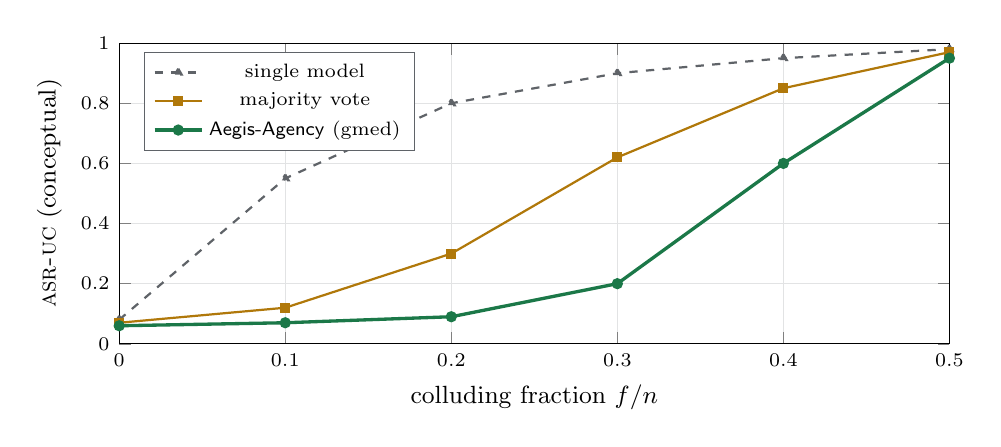
\begin{tikzpicture}
\begin{axis}[
    width=\textwidth, height=5.4cm,
    xlabel={colluding fraction $f/n$}, ylabel={\textsc{asr-uc} (conceptual)},
    xmin=0, xmax=0.5, ymin=0, ymax=1,
    xtick={0,0.1,0.2,0.3,0.4,0.5},
    legend style={at={(0.03,0.97)}, anchor=north west, font=\scriptsize, draw=aegisGray},
    tick label style={font=\scriptsize}, label style={font=\small},
    grid=both, grid style={aegisGray!18},
]
% single hardened model (no committee: fails once compromised)
\addplot[aegisGray, dashed, thick, mark=triangle*, mark size=1.4pt]
  coordinates {(0,0.08)(0.1,0.55)(0.2,0.8)(0.3,0.9)(0.4,0.95)(0.5,0.98)};
\addlegendentry{single model}
% plain majority vote
\addplot[aegisAmber, thick, mark=square*, mark size=1.4pt]
  coordinates {(0,0.07)(0.1,0.12)(0.2,0.3)(0.3,0.62)(0.4,0.85)(0.5,0.97)};
\addlegendentry{majority vote}
% Aegis (robust aggregation): flat until tolerance boundary, then rises
\addplot[aegisGreen, very thick, mark=*, mark size=1.4pt]
  coordinates {(0,0.06)(0.1,0.07)(0.2,0.09)(0.3,0.2)(0.4,0.6)(0.5,0.95)};
\addlegendentry{\Aegis\ (gmed)}
\end{axis}
\end{tikzpicture}
\caption{Evasion vs.\ colluding fraction.}
\label{fig:results-a}
\end{subcaptionblock}
\hfill
\begin{subcaptionblock}{0.49\textwidth}
\centering
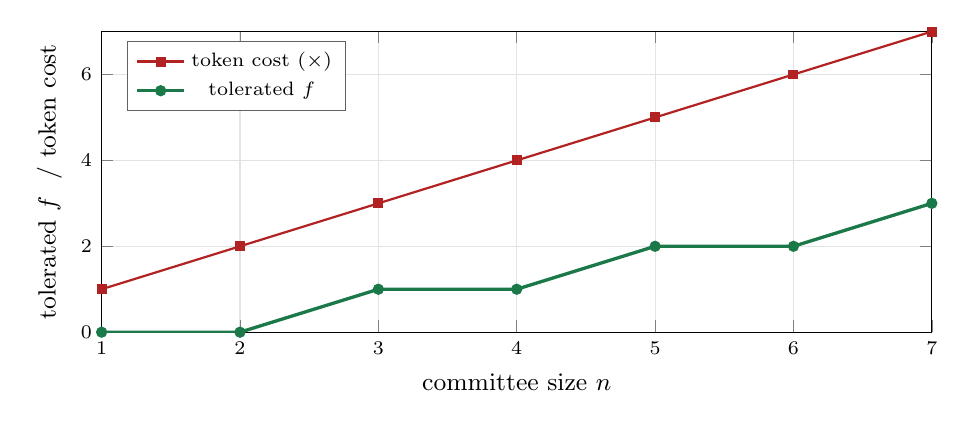
\begin{tikzpicture}
\begin{axis}[
    width=\textwidth, height=5.4cm,
    xlabel={committee size $n$}, ylabel={tolerated $f$ \ /\ token cost},
    xmin=1, xmax=7, ymin=0, ymax=7,
    xtick={1,2,3,4,5,6,7},
    legend style={at={(0.03,0.97)}, anchor=north west, font=\scriptsize, draw=aegisGray},
    tick label style={font=\scriptsize}, label style={font=\small},
    grid=both, grid style={aegisGray!18},
]
% token cost = n (linear)
\addplot[aegisRed, thick, mark=square*, mark size=1.4pt]
  coordinates {(1,1)(2,2)(3,3)(4,4)(5,5)(6,6)(7,7)};
\addlegendentry{token cost ($\times$)}
% tolerated faults floor((n-1)/2)
\addplot[aegisGreen, very thick, mark=*, mark size=1.4pt]
  coordinates {(1,0)(2,0)(3,1)(4,1)(5,2)(6,2)(7,3)};
\addlegendentry{tolerated $f$}
\end{axis}
\end{tikzpicture}
\caption{Security--cost frontier.}
\label{fig:results-b}
\end{subcaptionblock}
\caption{\textbf{Conceptual expected trends; not experimental results.} \emph{Placeholder
curves; replace with actual experimental data before submission.} (a)~Expected evasion
(\textsc{asr-uc}) as the colluding fraction grows: a single model fails as soon as it is
compromised, majority vote degrades earlier, and robust aggregation is expected to stay low
until the tolerance boundary $f<n/2$ before rising (graceful degradation, G3). (b)~The
security--cost frontier of \cref{tab:cost}: token cost grows linearly in $n$ while tolerated
faults grow as $\lfloor(n-1)/2\rfloor$. Shapes are illustrative, contain no measured data,
and encode the hypotheses the evaluation will test.}
\label{fig:results}
\end{figure}


\begin{table}[t]
\centering
\caption{\emph{Placeholder / expected-trend template; replace with measured results before
submission.} Main comparison at fixed diverse-backbone committee. Lower \textsc{asr-uc} and
\textsc{orr} are better. No numbers are filled because none have been measured.}
\label{tab:main}
\small
\begin{tabular}{@{}lccccc@{}}
\toprule
Method & $n$ & \textsc{asr-uc}$(f{=}1)$ & \textsc{asr-uc}$(f{=}2)$ & \textsc{orr} & Tokens ($\times$) \\
\midrule
Single hardened model~\cite{chen2025secalign} & 1 & -- & n/a & -- & $1$ \\
AutoDefense (single coord.)~\cite{zeng2024autodefense} & 3 & -- & -- & -- & $3$ \\
Plain majority vote & 5 & -- & -- & -- & $5$ \\
\Aegis\ ($\cmed$) & 5 & -- & -- & -- & $5$ \\
\Aegis\ ($\gmed$) & 5 & -- & -- & -- & $5$ \\
\Aegis\ ($\Krum$) & 5 & -- & -- & -- & $5$ \\
\bottomrule
\end{tabular}
\end{table}

\begin{table}[t]
\centering
\caption{\emph{Placeholder / expected-trend template; replace with measured results before
submission.} Ablation over the four components; each row disables one mechanism relative to
full \Aegis. Cells are intentionally empty.}
\label{tab:ablation}
\small
\begin{tabular}{@{}lcccc@{}}
\toprule
Configuration & Robust agg.\ & Isolation & Hardened judges & \textsc{asr-uc}$(f{=}1)$ \\
\midrule
Full \Aegis & \checkmark & \checkmark & \checkmark & -- \\
$-$ robust aggregation (single coord.) & & \checkmark & \checkmark & -- \\
$-$ payload isolation & \checkmark & & \checkmark & -- \\
$-$ hardened judges & \checkmark & \checkmark & & -- \\
$-$ all (AutoDefense-like) & & & & -- \\
\bottomrule
\end{tabular}
\end{table}

\section{Discussion}
\label{sec:discussion}

\paragraph{What the guarantees do and do not deliver.}
\Cref{thm:integrity} shows that robust verdict aggregation converts a Byzantine minority
into a bounded, and under a sufficient margin harmless, perturbation of the decision. The
force of the result is entirely in its condition $\gamma>C_\alpha r$: it moves the burden
of proof from ``is the pipeline secure?'' to the measurable ``do honest judges concentrate
tightly relative to their distance from the policy boundary?'' This is progress precisely
because it is falsifiable—$r$, $\gamma$, and $\rho$ are quantities \cref{sec:experiments}
measures, and a deployment in which honest judges are diffuse or the margin is small will
show it in those numbers rather than in a surprise failure.

\paragraph{Why aggregation in the verdict space, not over decisions.}
Plain majority vote is the natural committee baseline, but it aggregates only $d_k$ and is
therefore blind to a colluder that votes with the honest majority while manipulating scores
or rationales—to bias a downstream threshold, to poison an audit trail, or to prepare a
later escalation. Aggregating $(\score_k,\emb_k)\in\R^d$ makes such a colluder a geometric
outlier that $\gmed$ and $\Krum$ down-weight or reject. The cost is that the verdict space
must be well-behaved: the rationale embedding must place honest justifications near one
another and manipulated ones far away, which is an assumption on the encoder that we make
explicit and test, not one we take for granted.

\paragraph{Connection to robust learning, and its warning.}
We deliberately import machinery whose limits are documented. Adaptive attacks defeat
Krum and median in federated learning when the attacker stays within the honest
variance~\cite{baruch2019little,fang2020poisoning,xie2019fall}, and single-selection rules
degrade in high dimension~\cite{mhamdi2018bulyan}. Both warnings transfer. The first is why
our evaluation is adaptive by construction and why \cref{thm:integrity} is stated as a
conditional guarantee rather than an unconditional one; a colluding committee that keeps its
verdicts within the honest radius $r$ does not violate the theorem but does enlarge the
effective $r$, and that enlargement is exactly what the colluding-fraction sweep measures.
The second is why we keep the verdict space low-dimensional and treat $\Krum$ as one option
among three.

\paragraph{Diversity is a requirement, not a tuning knob.}
\Cref{prop:correlated} is the least comfortable result in the paper and the most important:
once honest errors are correlated, adding judges stops helping, and in the limit of
identical failure the committee is a single point of failure with a larger bill. Backbone
and prompt diversity is the only lever that reduces $\rho$, and the ensemble literature
cautions that diversity does not translate cleanly into
accuracy~\cite{kuncheva2003diversity}. We therefore report $\rho$ alongside every
robustness number and treat the homogeneous-vs-diverse gap as a headline measurement rather
than an ablation footnote.

\paragraph{Relation to the broader multi-agent security agenda.}
Recent work shows task-performing agent teams are attackable through their
interactions~\cite{lee2024promptinfection,he2025redteaming,ju2024flooding,zhou2025corba,zhang2024psysafe,zhang2024asb}.
\Aegis addresses the mirror-image problem for a \emph{defensive} team and, by using a star
topology with no inter-agent messages, removes the communication channel those attacks
exploit—at the cost of forgoing the benefits of agent debate~\cite{du2023debate}. Whether
a debating defense committee could achieve tighter honest concentration (smaller $r$)
without reopening the communication surface is an open question our architecture is
positioned to study but does not resolve.

\section{Limitations}
\label{sec:limitations}

We state the limitations plainly; several are structural and bound what the approach can
claim.

\paragraph{Conditional, not unconditional, guarantees.}
\Cref{thm:integrity} holds only when honest judges concentrate ($r$ small) and the decision
margin is large ($\gamma>C_\alpha r$). Neither is guaranteed in deployment: ambiguous
payloads, shared systematic biases~\cite{zheng2023judging,wang2023notfair}, and
near-boundary policies can violate both. The theorem does not certify security; it converts
security into measurable preconditions.

\paragraph{Small committees tolerate few faults.}
With $n\in\{3,4,5\}$ the tolerance is $f\in\{1,1,2\}$ (\cref{tab:cost}). Whether tolerating
a single compromised judge is meaningful robustness for a given deployment is an empirical
and threat-model question, not one the theory settles. Large committees are the natural
answer but multiply token and latency cost linearly (\cref{sec:complexity}).

\paragraph{Correlated failure is mitigated, not solved.}
\Cref{prop:correlated} shows that once honest errors are correlated, added judges stop
helping; diversity reduces but does not eliminate $\rho$, and the required diversity may be
hard to achieve when strong judges cluster on a few backbones. The limiting case of
identical failure across all judges is explicitly out of scope.

\paragraph{Adaptive attacks may enlarge the effective radius.}
A colluding committee that keeps its verdicts within the honest spread does not break
\cref{thm:integrity} but enlarges the effective $r$, and history shows adaptive attackers
find such
strategies against robust aggregators~\cite{baruch2019little,fang2020poisoning,xie2019fall}.
Our evaluation is adaptive, but no finite adaptive suite proves robustness against all
future attacks.

\paragraph{Isolation leakage is empirical.}
\Cref{prop:isolation} is conditional on the measured leakage $\varepsilon$; perfect
isolation is an idealisation. A judge whose fine-tuning is imperfect will have
$\varepsilon>0$, reopening a fraction of the second-order surface.

\paragraph{Embedding-space assumptions.}
Aggregating rationale embeddings assumes the encoder separates honest from manipulated
justifications; a colluder that produces honest-looking rationales for a dishonest verdict
stresses this assumption, and encoder robustness is itself an attack surface we do not fully
characterise.

\paragraph{Placeholder evaluation.}
The reported tables and plots are protocol templates, not measurements. Every quantitative
claim about \Aegis's effectiveness is therefore pending the experiments of
\cref{sec:experiments}; the contribution at this stage is the threat model, architecture,
and analysis, together with a falsifiable evaluation plan.

\section{Conclusion}
\label{sec:conclusion}

Multi-agent pipelines that filter LLM outputs have made the content they inspect safer
while leaving themselves unexamined. We argued that such a pipeline is a multi-agent system
whose own security matters, and we studied two threats with no single-model analogue:
compromised or colluding internal defenders, and second-order prompt injection carried by
the content the judges read. \Aegis answers both by replacing the single trusted
coordinator with Byzantine-robust aggregation of judge verdicts, isolating the untrusted
payload from the judges' instruction channel, hardening each judge, and generalising the
verdict target from jailbreak to task-integrity. We proved, under stated
honest-concentration and margin assumptions, that robust aggregation prevents a Byzantine
minority ($2f{+}2<n$ for selection, $f<n/2$ for median rules) from flipping the aggregate
decision in either direction; we characterised how the guarantee degrades once honest
failures correlate, turning backbone diversity from a tuning choice into a requirement; and
we quantified the linear token/latency cost the committee incurs. We were explicit
throughout that a lower attack success rate under compromise is evidence of graceful
degradation, not a proof of security, and that the empirical figures here are placeholders
fixing a falsifiable protocol.

Two directions follow directly. First, executing the adaptive evaluation of
\cref{sec:experiments}—especially the homogeneous-vs-diverse correlated-failure test and the
security-versus-cost frontier—will tell us whether the preconditions of \cref{thm:integrity}
hold for real hardened LLM judges, which is the crux of whether the approach is practically
meaningful at small $n$. Second, tightening honest concentration without reopening the
inter-agent communication surface—for instance through structured, non-adversarial
consensus among judges—could relax the margin condition and extend tolerance, and is a
question the star-topology architecture is positioned to study. We hope the framing of the
defense pipeline as a first-class attack surface, and the insistence on stating exactly
where robustness stops, are useful beyond the specific architecture proposed here.


% ---------------------------------------------------------------------
\appendix
\section{Proofs}
\label{app:proofs}

This appendix gives the complete proofs of the results marked complete in \cref{sec:theory}
and the deferred specialisations of the sketched results.

\subsection{Proof of \cref{lem:gmedrobust} (geometric-median displacement)}
\begin{proof}
Let $\uhat=\arg\min_{\bm y\in\R^d} F(\bm y)$ with $F(\bm y)=\sum_{k=1}^n\lVert \bm
y-\verd_k\rVert$, the geometric median. Optimality gives $F(\uhat)\le F(\ustar)$, i.e.
\begin{equation}
  \sum_{k\in\Hset}\lVert\uhat-\verd_k\rVert + \sum_{k\in\Bset}\lVert\uhat-\verd_k\rVert
  \;\le\;
  \sum_{k\in\Hset}\lVert\ustar-\verd_k\rVert + \sum_{k\in\Bset}\lVert\ustar-\verd_k\rVert .
  \label{eq:opt}
\end{equation}
Rearranging \cref{eq:opt},
\begin{equation}
  \sum_{k\in\Hset}\bigl(\lVert\uhat-\verd_k\rVert-\lVert\ustar-\verd_k\rVert\bigr)
  \;\le\;
  \sum_{k\in\Bset}\bigl(\lVert\ustar-\verd_k\rVert-\lVert\uhat-\verd_k\rVert\bigr).
  \label{eq:rearr}
\end{equation}
For the right-hand side, the reverse triangle inequality gives, for every $k$,
$\lVert\ustar-\verd_k\rVert-\lVert\uhat-\verd_k\rVert\le\lVert\ustar-\uhat\rVert$, hence
\begin{equation}
  \text{RHS of \eqref{eq:rearr}} \;\le\; |\Bset|\,\lVert\ustar-\uhat\rVert = f\,\lVert\uhat-\ustar\rVert.
  \label{eq:rhs}
\end{equation}
For the left-hand side, fix an honest $k\in\Hset$. By the triangle inequality
$\lVert\uhat-\verd_k\rVert\ge\lVert\uhat-\ustar\rVert-\lVert\ustar-\verd_k\rVert$, and since
$\lVert\ustar-\verd_k\rVert\le r$ (\cref{ass:concentration}),
\begin{equation}
  \lVert\uhat-\verd_k\rVert-\lVert\ustar-\verd_k\rVert
  \;\ge\; \lVert\uhat-\ustar\rVert - \lVert\ustar-\verd_k\rVert - \lVert\ustar-\verd_k\rVert
  \;\ge\; \lVert\uhat-\ustar\rVert - 2r .
  \label{eq:lhsterm}
\end{equation}
Summing \cref{eq:lhsterm} over the $|\Hset|=n-f$ honest judges,
\begin{equation}
  \text{LHS of \eqref{eq:rearr}} \;\ge\; (n-f)\bigl(\lVert\uhat-\ustar\rVert-2r\bigr).
  \label{eq:lhs}
\end{equation}
Combining \cref{eq:rhs,eq:lhs} with \cref{eq:rearr},
\begin{equation}
  (n-f)\bigl(\lVert\uhat-\ustar\rVert-2r\bigr)\;\le\; f\,\lVert\uhat-\ustar\rVert
  \;\;\Longrightarrow\;\;
  (n-2f)\,\lVert\uhat-\ustar\rVert \;\le\; 2(n-f)\,r .
\end{equation}
Since $f<n/2$ we have $n-2f>0$, so dividing yields
$\lVert\uhat-\ustar\rVert\le \frac{2(n-f)}{n-2f}\,r = C_\alpha r$ with
$\alpha=f/n$. The Byzantine verdicts entered only through \cref{eq:rhs}, where the bound is
independent of their values, so the displacement bound holds for arbitrary Byzantine
$\{\verd_k\}_{k\in\Bset}$. \qedhere
\end{proof}

\begin{remark}
The constant $C_\alpha=\tfrac{2(1-\alpha)}{1-2\alpha}$ is a \emph{sufficient} displacement
bound, consistent with the breakdown point $\tfrac12$ of the geometric
median~\cite{lopuhaa1991breakdown,minsker2015geometric}. We make no optimality or matching
claim: a smaller constant may hold under additional assumptions, and the divergence as
$\alpha\to\tfrac12$ is intrinsic to any minority-tolerance estimator.
\end{remark}

\subsection{Proof of \cref{thm:integrity} (decision integrity)}
\begin{proof}
By \cref{lem:gmedrobust} (for $\gmed$) the aggregate satisfies
$\lVert\uhat-\ustar\rVert\le C_\alpha r$. The score coordinate is a $1$-Lipschitz
projection, $|\pi_1(\uhat)-\pi_1(\ustar)|\le\lVert\uhat-\ustar\rVert\le C_\alpha r$. By
\cref{ass:margin}, $\pi_1(\ustar)$ lies at distance at least $\gamma$ from the threshold
$\thr$. If $\gamma>C_\alpha r$ (\cref{eq:integritycond}), then $\pi_1(\uhat)$ stays on the
same side of $\thr$ as $\pi_1(\ustar)$:
\begin{equation}
  \pi_1(\ustar)\ge\thr+\gamma \Rightarrow \pi_1(\uhat)\ge \thr+\gamma-C_\alpha r>\thr,
  \qquad
  \pi_1(\ustar)\le\thr-\gamma \Rightarrow \pi_1(\uhat)\le \thr-\gamma+C_\alpha r<\thr .
\end{equation}
Hence $\dec(\uhat)=\mathbf 1\{\pi_1(\uhat)\ge\thr\}=\mathbf 1\{\pi_1(\ustar)\ge\thr\}
=\dec(\ustar)=y^\star(\pay)$, for every choice of the Byzantine verdicts. Both directions
are covered: the payload the honest committee would block is blocked (no forced pass), and
the one it would allow is allowed (no forced block). \qedhere
\end{proof}

\begin{proof}[Proof of \cref{cor:availability}]
The two implications in the proof of \cref{thm:integrity} are symmetric in the sign of
$\pi_1(\ustar)-\thr$; the second implication is exactly the statement that a benign payload
($\pi_1(\ustar)\le\thr-\gamma$, so $\dec(\ustar)=0$) cannot be pushed to $\hat d=1$ by the
Byzantine judges. \qedhere
\end{proof}

\subsection{Proof of \cref{prop:cmed} (coordinate-wise median)}
\begin{proof}
Fix a coordinate $j$ and consider the $n$ scalars $\{\pi_j(\verd_k)\}_{k\in[n]}$, of which
at most $f$ are Byzantine. Let $a=\min_{k\in\Hset}\pi_j(\verd_k)$ and
$b=\max_{k\in\Hset}\pi_j(\verd_k)$ be the honest range. Among all $n$ values, at least
$n-f>n/2$ lie in $[a,b]$. A median (any order statistic of rank $\lceil n/2\rceil$ or
$\lfloor n/2\rfloor+1$) of $n$ numbers of which strictly more than half lie in $[a,b]$ must
itself lie in $[a,b]$: fewer than $n/2$ values lie strictly below $a$ and fewer than $n/2$
strictly above $b$, so the middle order statistic is bracketed. Thus
$\pi_j(\uhat)\in[a,b]$. For $j=1$ (score), $a,b\in[\pi_1(\ustar)-r,\pi_1(\ustar)+r]$ by
\cref{ass:concentration}, giving $|\pi_1(\uhat)-\pi_1(\ustar)|\le r$. Substituting the
displacement $r$ (i.e.\ $C_\alpha=1$) into the margin argument of \cref{thm:integrity}
yields the decision guarantee whenever $\gamma>r$. \qedhere
\end{proof}

\subsection{Proof of \cref{prop:isolation} (isolation containment)}
\begin{proof}
Fix an honest judge $k$ with verdict law $P_k(\cdot\mid c,\pay)$. Its decision is the event
$A=\{v:\dec=1\}$. By $\varepsilon$-isolation (\cref{def:isolation}),
$|P_k(A\mid c,\pay)-P_k(A\mid c,\pay')|\le\operatorname{TV}(P_k(\cdot\mid c,\pay),
P_k(\cdot\mid c,\pay'))\le\varepsilon$, so the injection changes judge $k$'s decision
probability by at most $\varepsilon$; the probability it flips a fixed drawn decision is at
most $\varepsilon$. If honest judges draw independently, the number of flipped honest
decisions is stochastically dominated by a $\mathrm{Binomial}(n-f,\varepsilon)$, whence
$\Prob[\text{more than }t\text{ flips}]\le\binom{n-f}{t+1}\varepsilon^{t+1}$ by the union
bound over $(t{+}1)$-subsets. When $\varepsilon=0$ every honest verdict law is invariant to
the injection, so no honest verdict changes and the attacker must instead corrupt judges
directly, which is a Byzantine action counted in $f$ and governed by \cref{thm:integrity}.
\qedhere
\end{proof}

\subsection{Proof of \cref{prop:correlated} (correlated honest failure)}
\begin{proof}
Let $\{Z_k\}_{k\in\Hset}$ be exchangeable Bernoulli$(\mu)$ with
$\operatorname{Corr}(Z_i,Z_j)=\rho$ for $i\ne j$, so
$\operatorname{Cov}(Z_i,Z_j)=\rho\,\mu(1-\mu)$. With $N=n-f$ and
$\bar Z=\frac1N\sum_{k}Z_k$,
\begin{equation}
  \operatorname{Var}(\bar Z)
  = \frac{1}{N^2}\Bigl(\sum_k\operatorname{Var}(Z_k) + \sum_{i\ne j}\operatorname{Cov}(Z_i,Z_j)\Bigr)
  = \frac{1}{N^2}\Bigl(N\mu(1-\mu) + N(N-1)\rho\,\mu(1-\mu)\Bigr),
\end{equation}
which simplifies to $\operatorname{Var}(\bar Z)=\mu(1-\mu)\bigl[\tfrac{1-\rho}{N}+\rho\bigr]$,
proving \cref{eq:corrvar}. As $N\to\infty$ the first term vanishes and
$\operatorname{Var}(\bar Z)\to\mu(1-\mu)\rho$, which is strictly positive for
$\rho\in(0,1]$ and $\mu\in(0,1)$; the sample mean does not concentrate at $\mu$. For the
majority-failure lower bound, a correct honest majority requires $\bar Z>\tfrac12$. If
$\mu\le\tfrac12$ then $\{\bar Z>\tfrac12\}\subseteq\{\bar Z-\mu>\tfrac12-\mu\}$ and, when
$\mu<\tfrac12$, Chebyshev gives
$\Prob[\bar Z>\tfrac12]\le \Prob[|\bar Z-\mu|\ge\tfrac12-\mu] \le
\frac{\operatorname{Var}(\bar Z)}{(\tfrac12-\mu)^2}$. As $N\to\infty$ this upper bound tends
to $\frac{\mu(1-\mu)\rho}{(\tfrac12-\mu)^2}$, a constant independent of $N$; hence for
$\rho>0$ the honest majority cannot be made correct with probability approaching one merely
by enlarging the committee. Reducing $\rho$ (through backbone/prompt diversity) is the only
term in \cref{eq:corrvar} that restores $1/N$-style concentration. \qedhere
\end{proof}

\begin{remark}
The bound is one-sided and asymptotic in $N$; it establishes that correlation imposes a
$\rho$-dependent floor on committee variance, which is the formal content of the idea's
``vacuous if all judges fail identically.'' It is a limiting-case impossibility for the
honest majority, not a defense, and we present it as such.
\end{remark}

\section{Additional Experimental Detail}
\label{app:experiments}

This appendix expands the protocol of \cref{sec:experiments}. As there, \textbf{all figures
and tables in this appendix are placeholders / expected trends and must be replaced with
measured results before submission.}

\subsection{Attacker instantiation}
For the \emph{colluding-defenders} attack we adopt the ``a-little-is-enough''
principle~\cite{baruch2019little}: the $f$ Byzantine judges each report a verdict vector
$\verd_k=\ustar+ z\,\hat{\bm g}$, where $\hat{\bm g}$ is the estimated direction toward the
decision boundary and $z\le r$ keeps each Byzantine verdict inside the honest radius so that
robust aggregation cannot flag it as an outlier. The colluding-fraction sweep increases $f$
until $2f{+}2<n$ is violated. For the \emph{adaptive-on-aggregation} attack we optimise
$\{\verd_k\}_{k\in\Bset}$ against the specific rule: inner-product
manipulation~\cite{xie2019fall} for $\gmed$/$\cmed$ and the local-model-poisoning
objective~\cite{fang2020poisoning} for $\Krum$. The \emph{second-order injection} attack
uses JudgeDeceiver~\cite{shi2024judgeinjection} to craft payload suffixes, evaluated with
isolation on and off to estimate $\varepsilon$ (\cref{def:isolation}).

\subsection{Measuring the theory's quantities}
\Cref{thm:integrity,prop:correlated} predict behaviour through $r$, $\gamma$, and $\rho$;
we measure all three. The honest radius $r$ is the empirical $95$th-percentile of
$\lVert\verd_k-\ustar\rVert$ over honest judges with $\ustar$ the honest geometric median.
The margin $\gamma$ is $|\pi_1(\ustar)-\thr|$ averaged over payloads, reported separately
for benign and adversarial classes. The correlation $\rho$ is the mean pairwise correlation
of honest correctness indicators, reported for homogeneous and diverse committees to test
RQ4. Plotting \textsc{asr-uc} against the measured $C_\alpha r/\gamma$ ratio provides a
direct check of \cref{eq:integritycond}: the theory predicts a rise in \textsc{asr-uc} as
$C_\alpha r/\gamma$ crosses $1$.

\subsection{Placeholder frontier and sweeps}
\Cref{fig:results} (main text) shows the two conceptual sweeps: \textsc{asr-uc} versus
colluding fraction, and the security--cost frontier versus $n$. Both are drawn as expected
trends with no data. The correlated-failure ablation is reported as paired
(homogeneous, diverse) points at each $n$, with $\rho$ annotated.

\subsection{Reproducibility artefacts}
On release we provide: backbone checkpoints/versions and decoding parameters; the isolation
delimiter scheme and per-request nonce generation; hardening (SecAlign/StruQ) training
configurations; aggregation tolerances ($\eta$, assumed $f$); attack budgets per benchmark;
seeds; and the payload manifests mapping each item to its source benchmark and ground-truth
label. Each released number carries its measurement conditions and dispersion across seeds.


% ---------------------------------------------------------------------
\bibliographystyle{elsarticle-num}
\bibliography{references_verified}

\end{document}
